

\chapter{Reglerentwruf und Versuchsdurchführung}\label{chap:versuch}
	\subsection*{Ermittlung der Kennlinie}
	Zur Ermittlung der Kennlinie wurde an 4 Punkten der Strom gemessen, bei welchem $F_g = F_{mag}$ galt und somit der Ball nach oben gezogen wurde.

	\begin{table}[!h]
			\renewcommand{\arraystretch}{1.2}
			\centering
			\caption{Tabelle zur Ermittlung der Kennlinie}
			\begin{zebratabular}{m{3cm} m{3cm}}
				\rowcolor{gray}
				\textbf{$x [m]$}	& \textbf{$i [A]$}		    \\
				$0.035$				& $0.398$  \\ 
				$0.040$				& $0.505$  \\
				$0.045$				& $0.6369$ \\
				$0.050$				& $0.8964$ \\
			\end{zebratabular}
			\renewcommand{\arraystretch}{1.0}
			\label{tab:kenn_strom}
		\end{table}
		Die Polynomfaktoren werden ebenfalls aus diesen Messungen bestimmt:
			\begin{figure}[H]
				\centering
				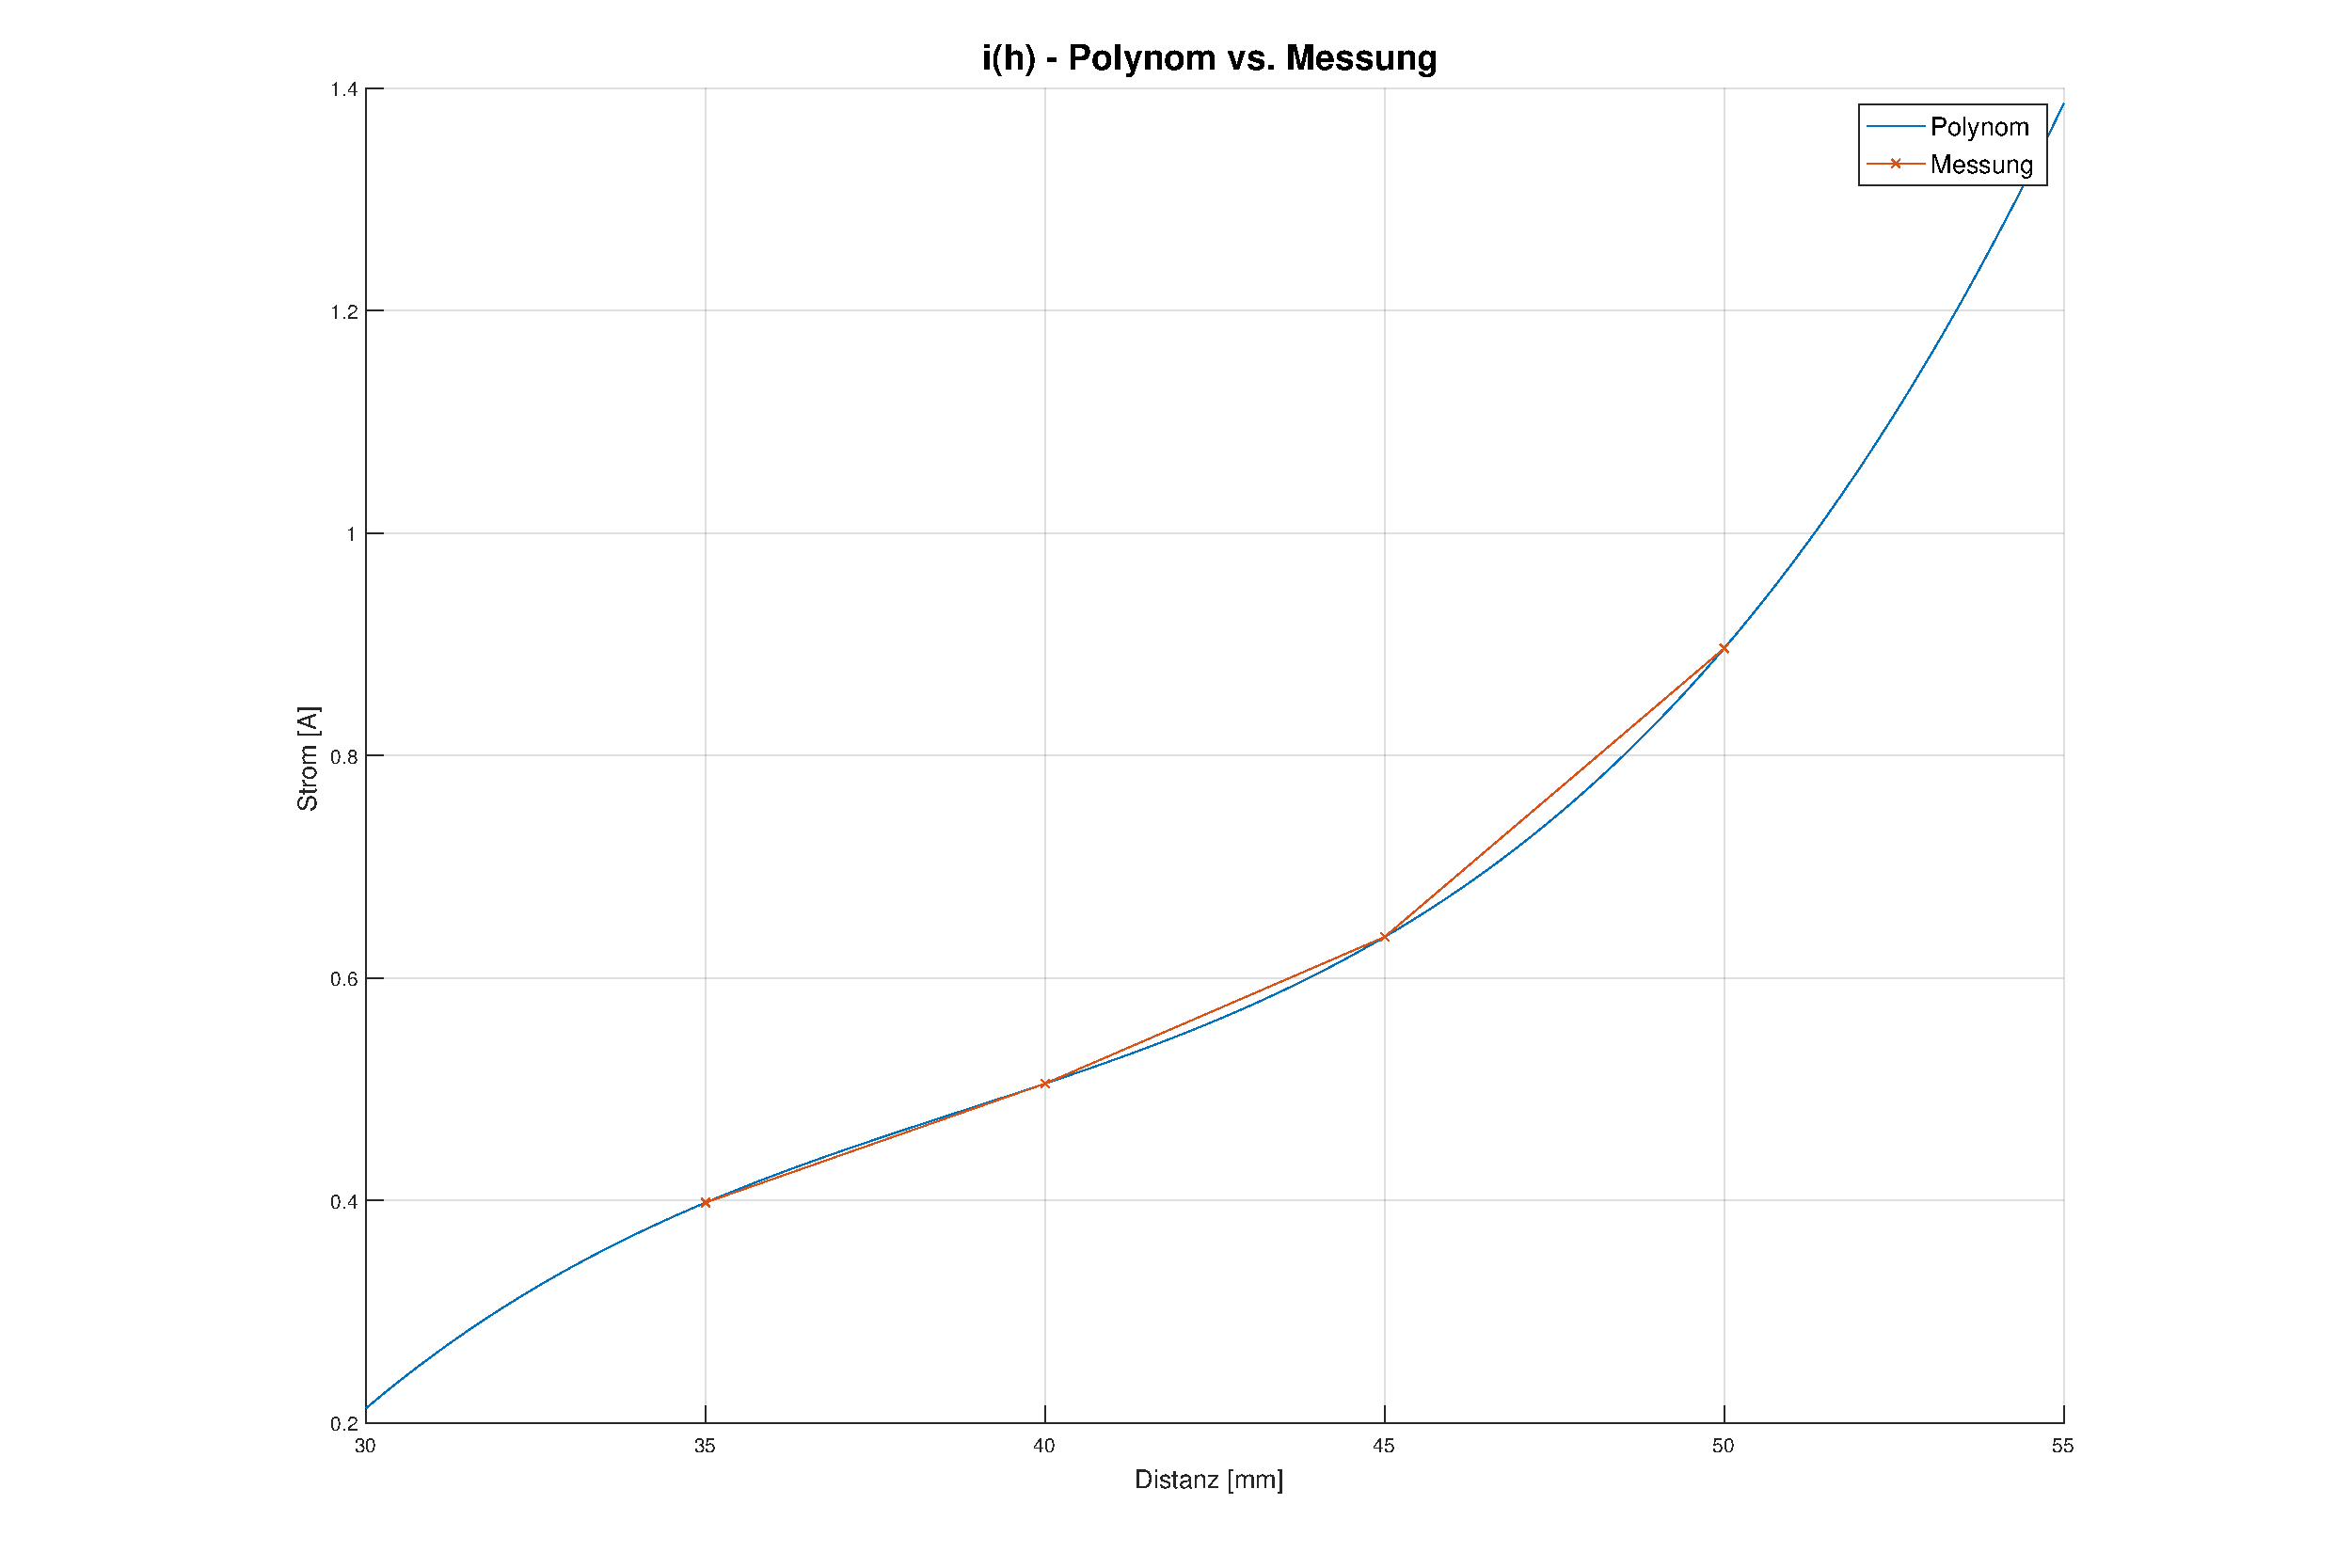
\includegraphics[width=.9\textwidth]{./figure/abstand_polyfit.pdf}
				\caption{Gemessene Punkte überlagert mit gefundenem Polynom}
				\label{fig:poly}
			\end{figure}
\newpage	
\section{Aufgabe 12}\label{sec:Aufgabe12}
	\subsection*{Vorzeichen der Reglerverstärkung}
	Das Vorzeichen von $K_{p}$ ist positiv.

\section{Aufgaben 13, 14 und 15}\label{sec:Aufgabe13_14}
	\subsection*{Wurzelortskurve des PD-Reglers}
	Durch Untersuchen der Wurzelortskurve (rlocus \autoref{fig:rlocusPD})  kann mit der Wahl von $T_d = \frac{1}{\sqrt{k_x}}$ erkannt werden, dass eine Verstärkung $K_p \geq 40$ nötig ist, um alle Pole in die negative Halbebene zu bewegen.
	\begin{figure}[H]
				\centering
				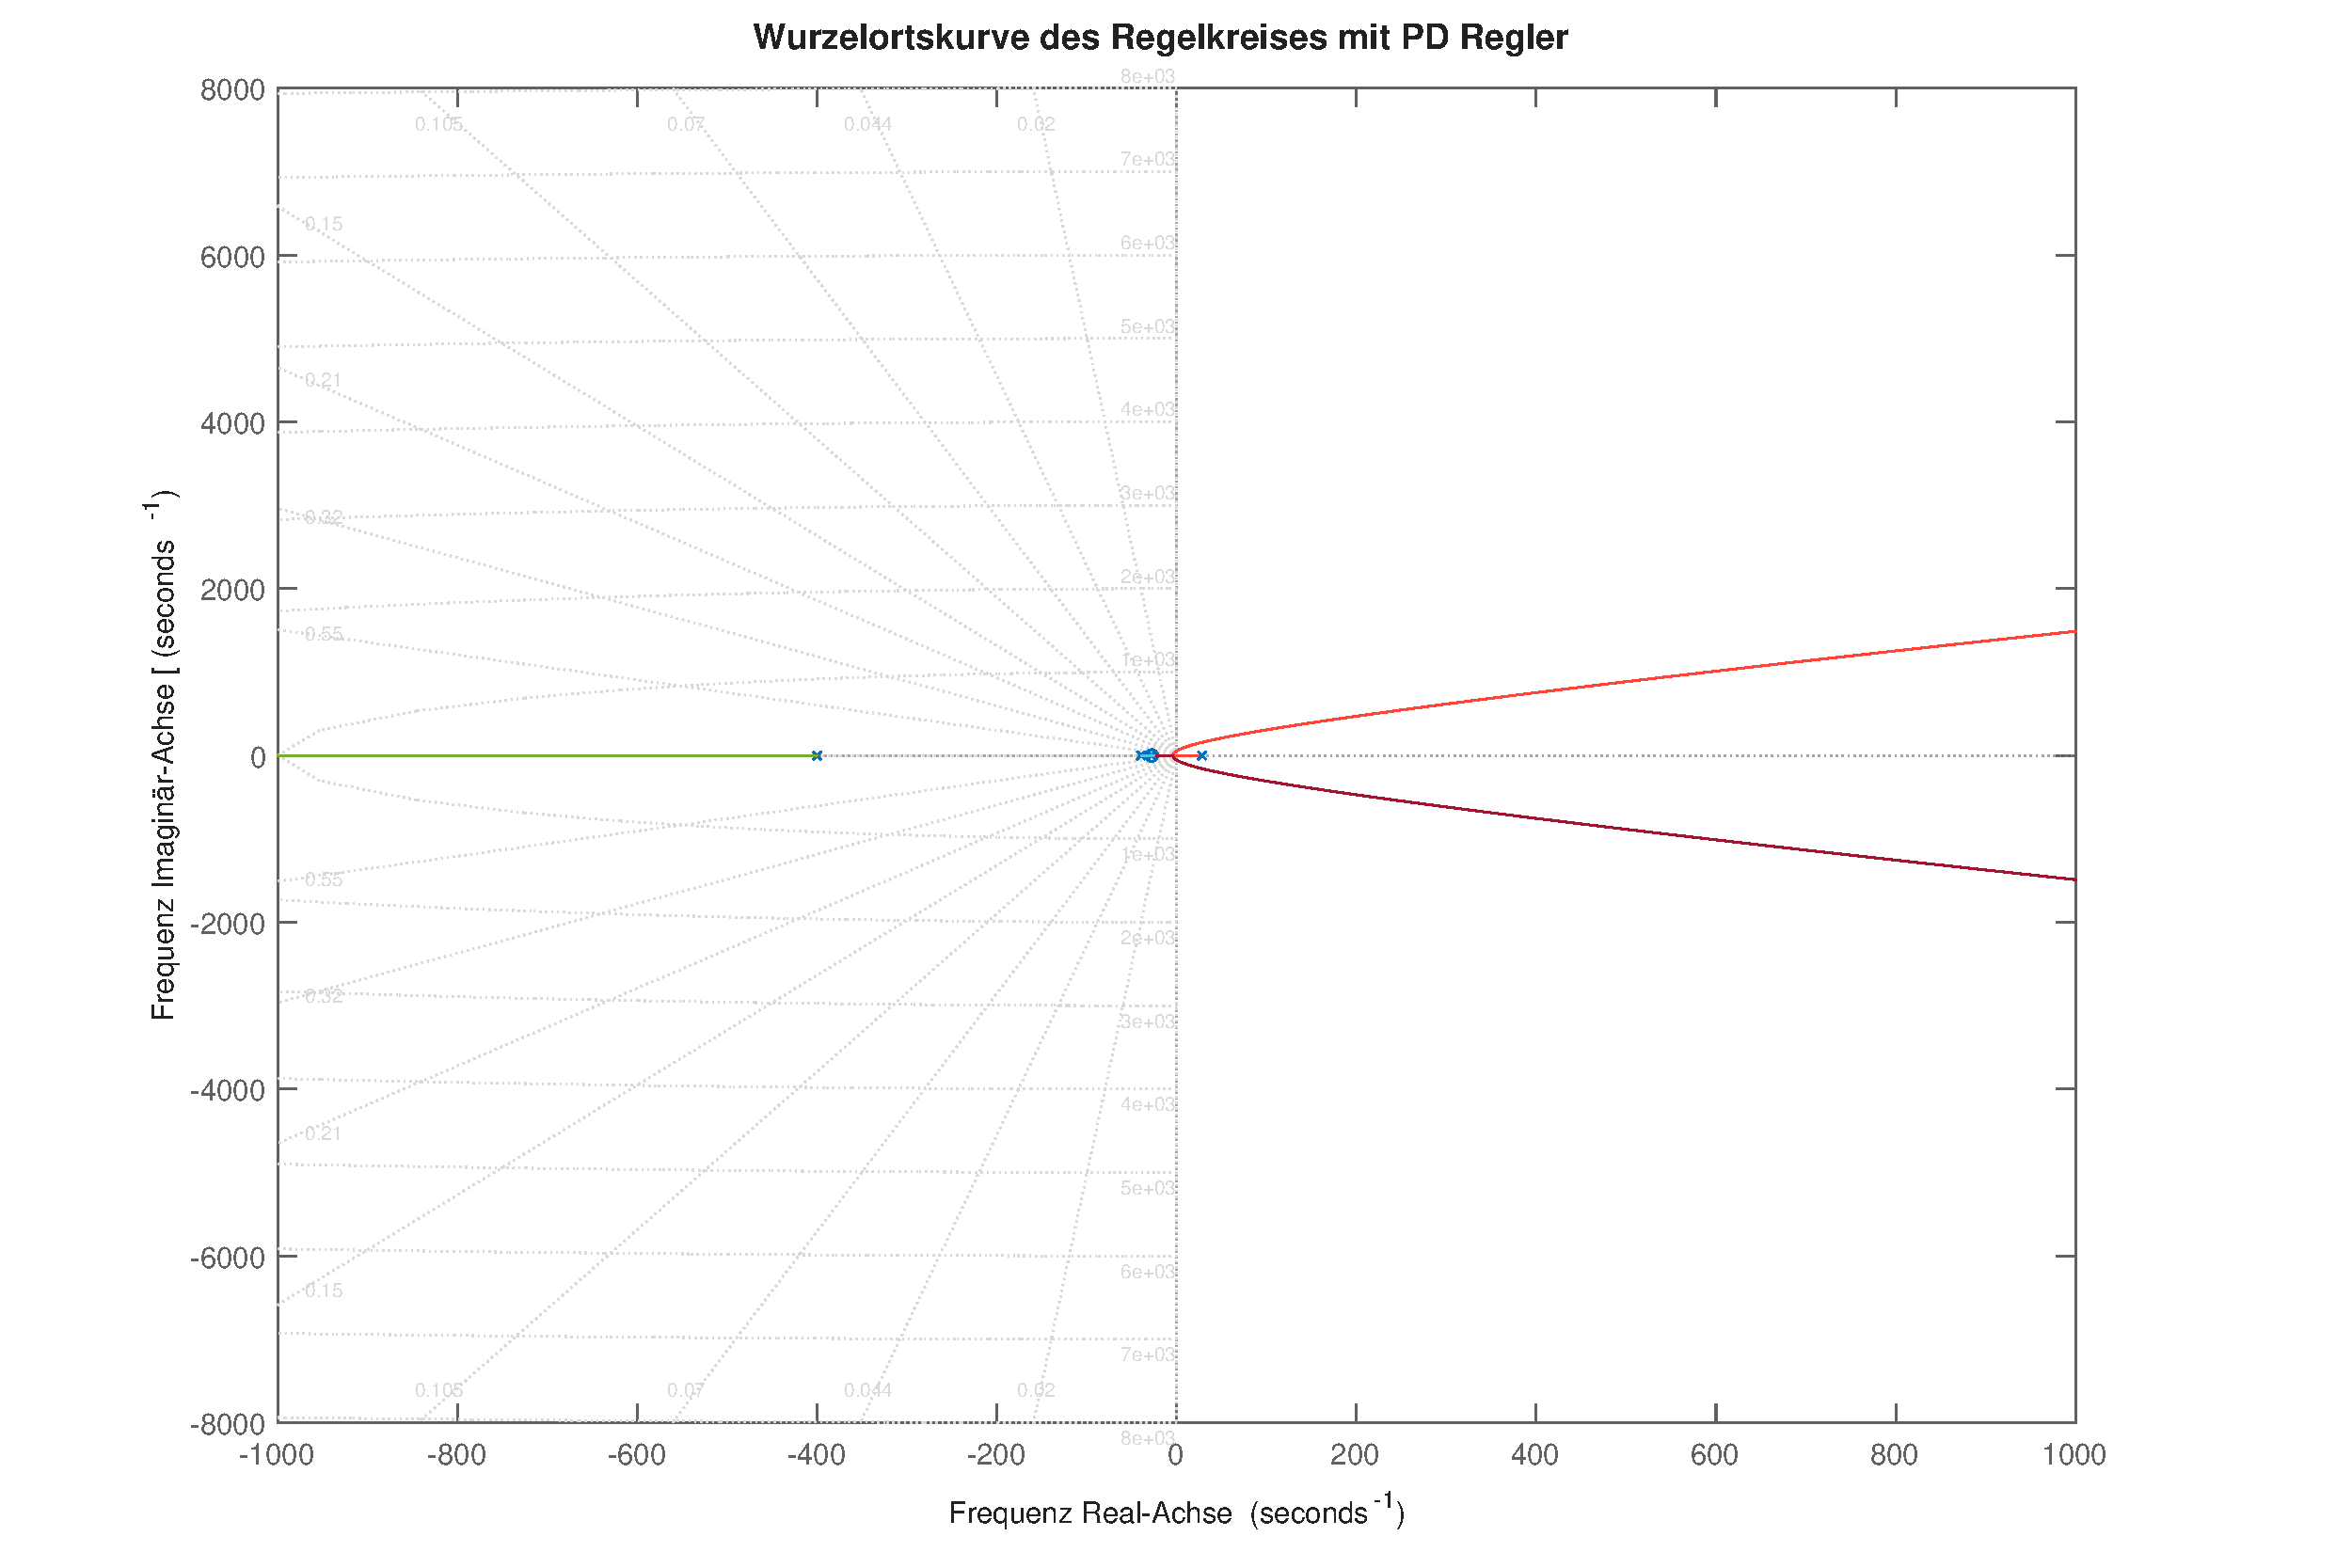
\includegraphics[width=.9\textwidth]{./figure/rlocus_pd_untuned.pdf}
				\caption{Wurzelortskurve des Prozesses mit PD-Regler}
				\label{fig:rlocusPD}
			\end{figure}


			Somit ergibt sich ein PD Regler $C_{PD} = K_p \cdot \left(  1 + T_d \frac{s}{\frac{N}{T_d}s + 1} \right)$ mit $K_p=40, T_d = \frac{1}{\sqrt{k_x}}$ und $N=100$.
			\newpage
			In \autoref{fig:polePD} ist erkenntlich, dass alle Pole in der linken (negativen) Halbebene liegen.

			\begin{figure}[H]
				\centering
				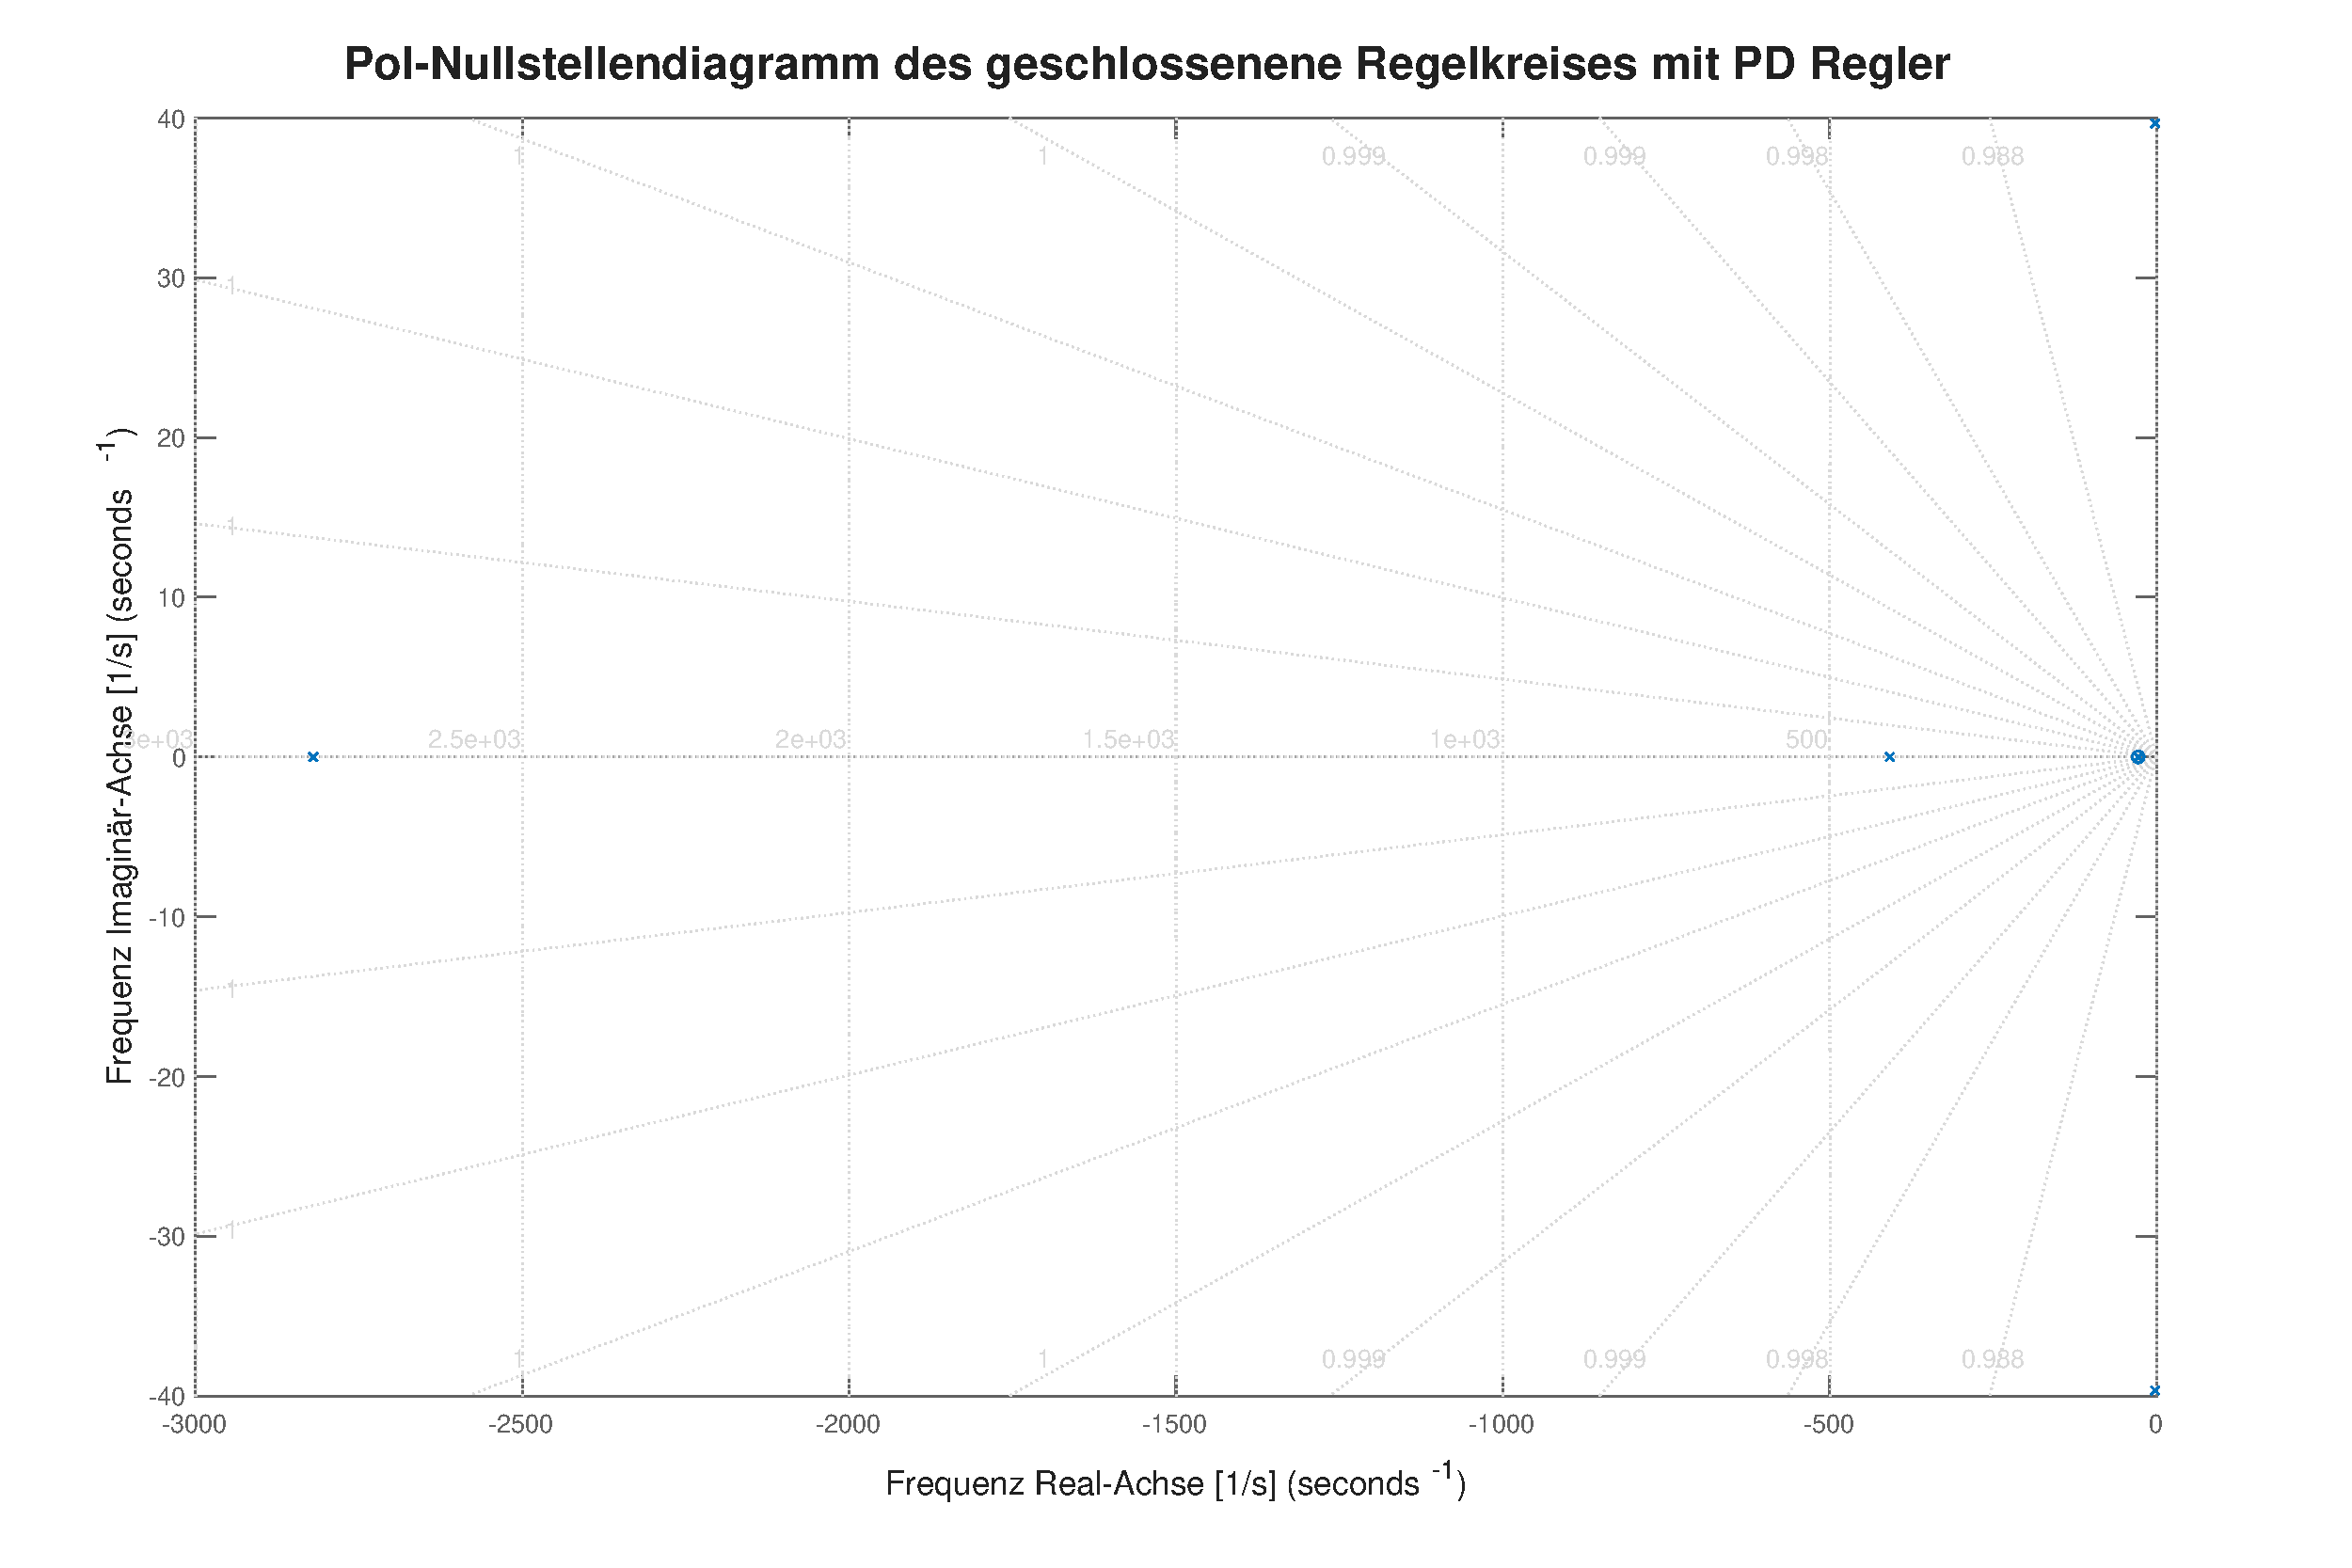
\includegraphics[width=.9\textwidth]{./figure/polemap_pd_untuned.pdf}
				\caption{Pole des Prozesses mit PD-Regler}
				\label{fig:polePD}
			\end{figure}
\newpage
	\subsection*{Erweiterung zum PID-Regler}
	Mit der gegebenen Vorschrift von $T_d < 0.25 T_i$ wurde zusammen mit Untersuchung der Wurzelortskurve ein Wert von $T_i = \frac{T_d}{T_i} + 0.1$ ermittelt.



	\begin{figure}[H]
				\centering
				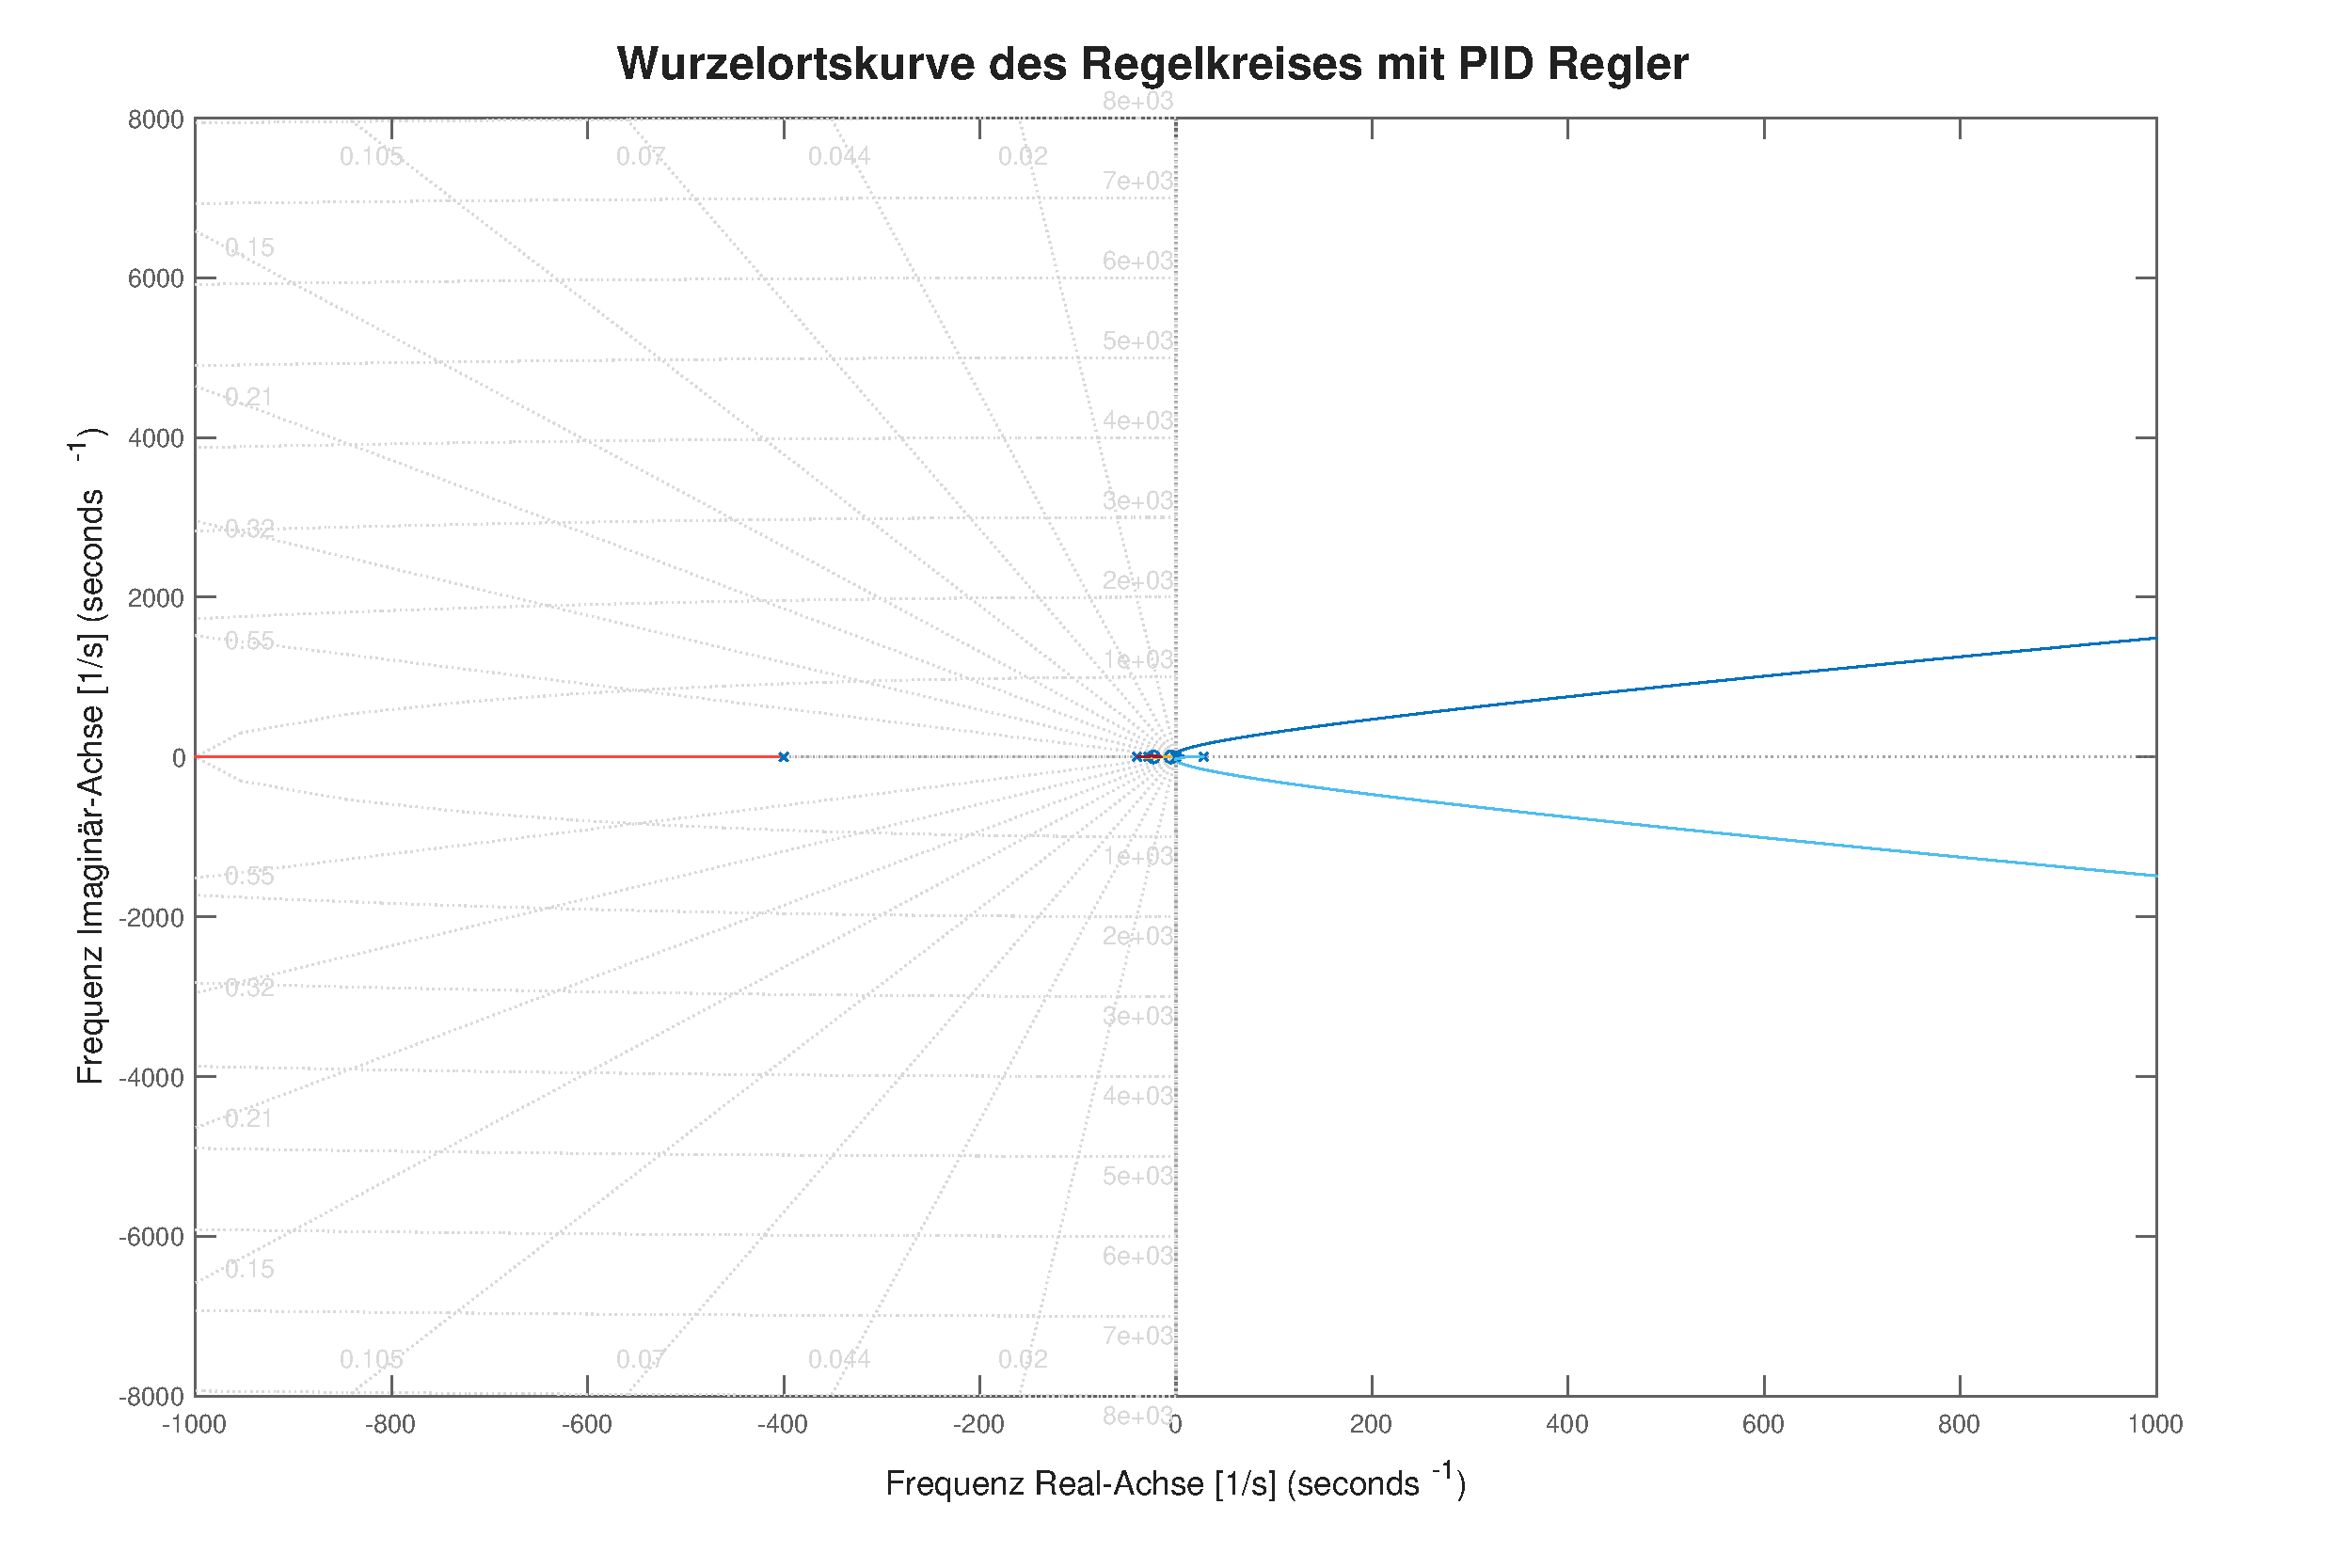
\includegraphics[width=.9\textwidth]{./figure/rlocus_pid_untuned.pdf}
				\caption{Wurzelortskurve des Prozesses mit PD-Regler}
				\label{fig:rlocusPID}
			\end{figure}


			Somit ergibt sich ein PID Regler $C_{PD} = K_p \cdot \left(  1 +\frac{1}{T_i}\cdot \frac{1}{s} + T_d \frac{s}{\frac{N}{T_d}s + 1} \right)$ mit $K_p=40, T_d = \frac{1}{\sqrt{k_x}}$ und $N=100$.
			\newpage
			In \autoref{fig:polePID} ist erkenntlich, dass alle Pole in der linken (negativen) Halbebene liegen.

			\begin{figure}[H]
				\centering
				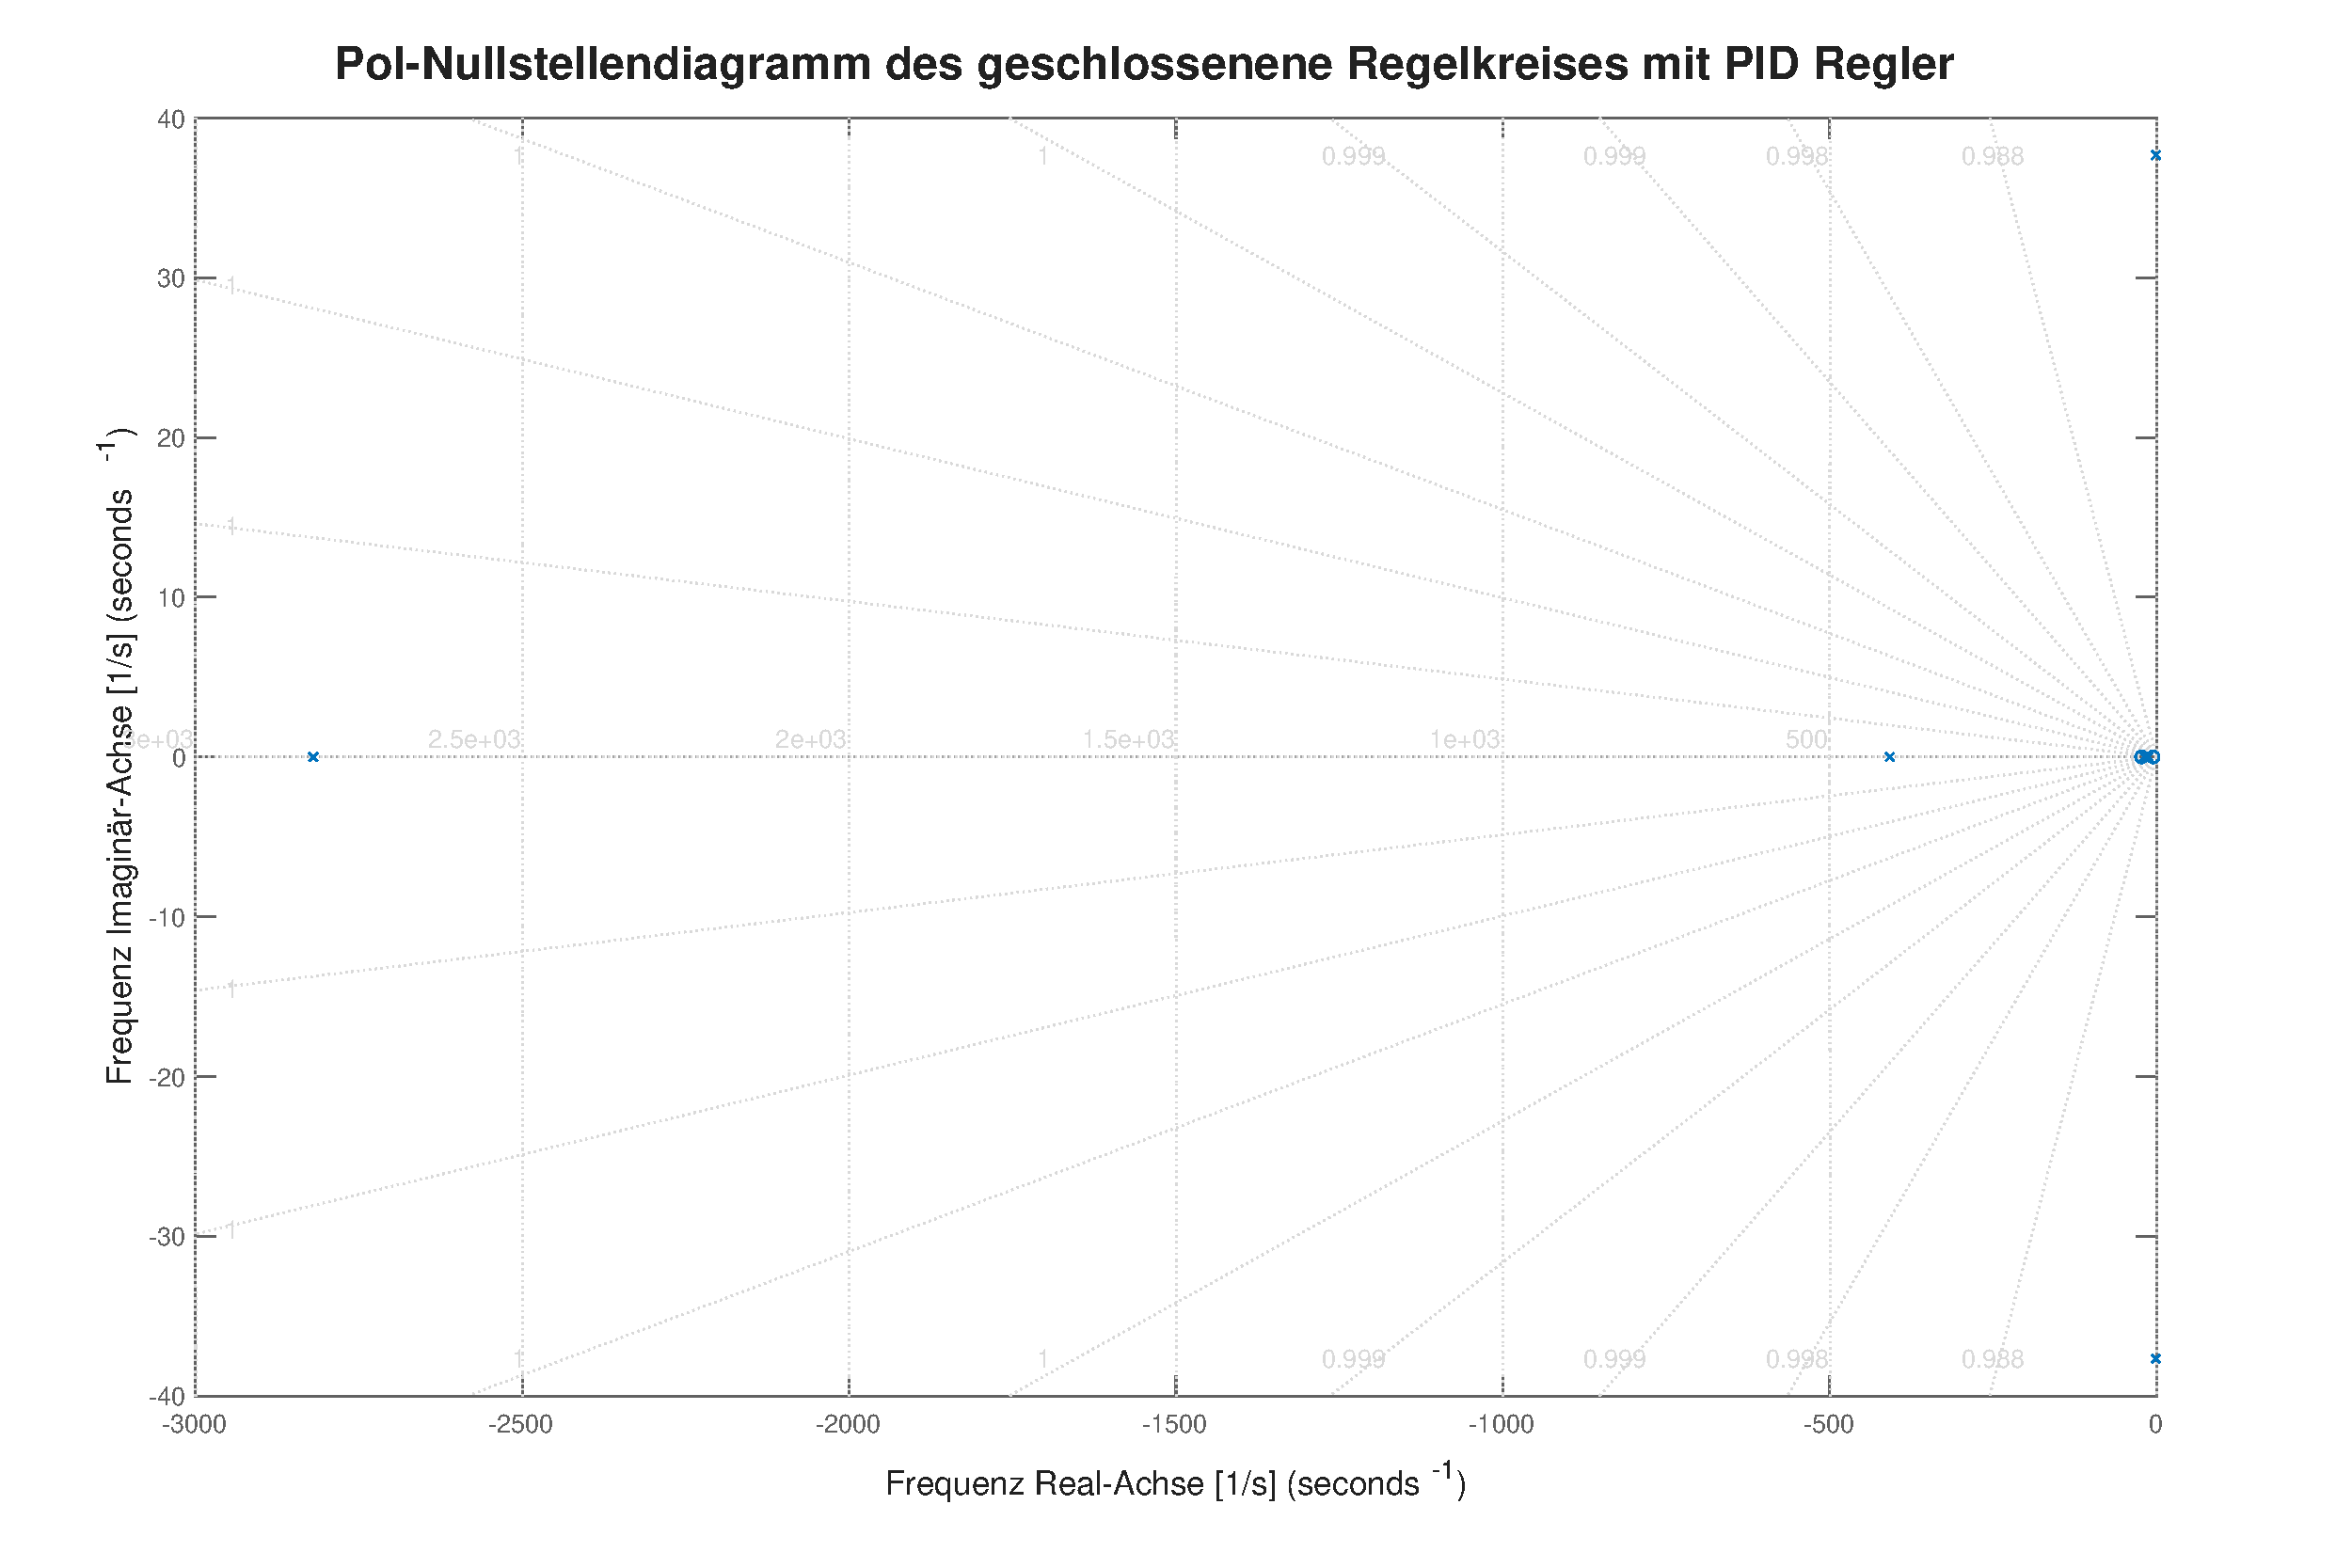
\includegraphics[width=.9\textwidth]{./figure/polemap_pid_untuned.pdf}
				\caption{Pole des Prozesses mit PID-Regler}
				\label{fig:polePID}
			\end{figure}


\newpage
\section{Aufgabe 16}\label{sec:Aufgabe16}
	\subsection*{Simulinkmodell des Aufbaus}
			\begin{figure}[H]
				\centering
				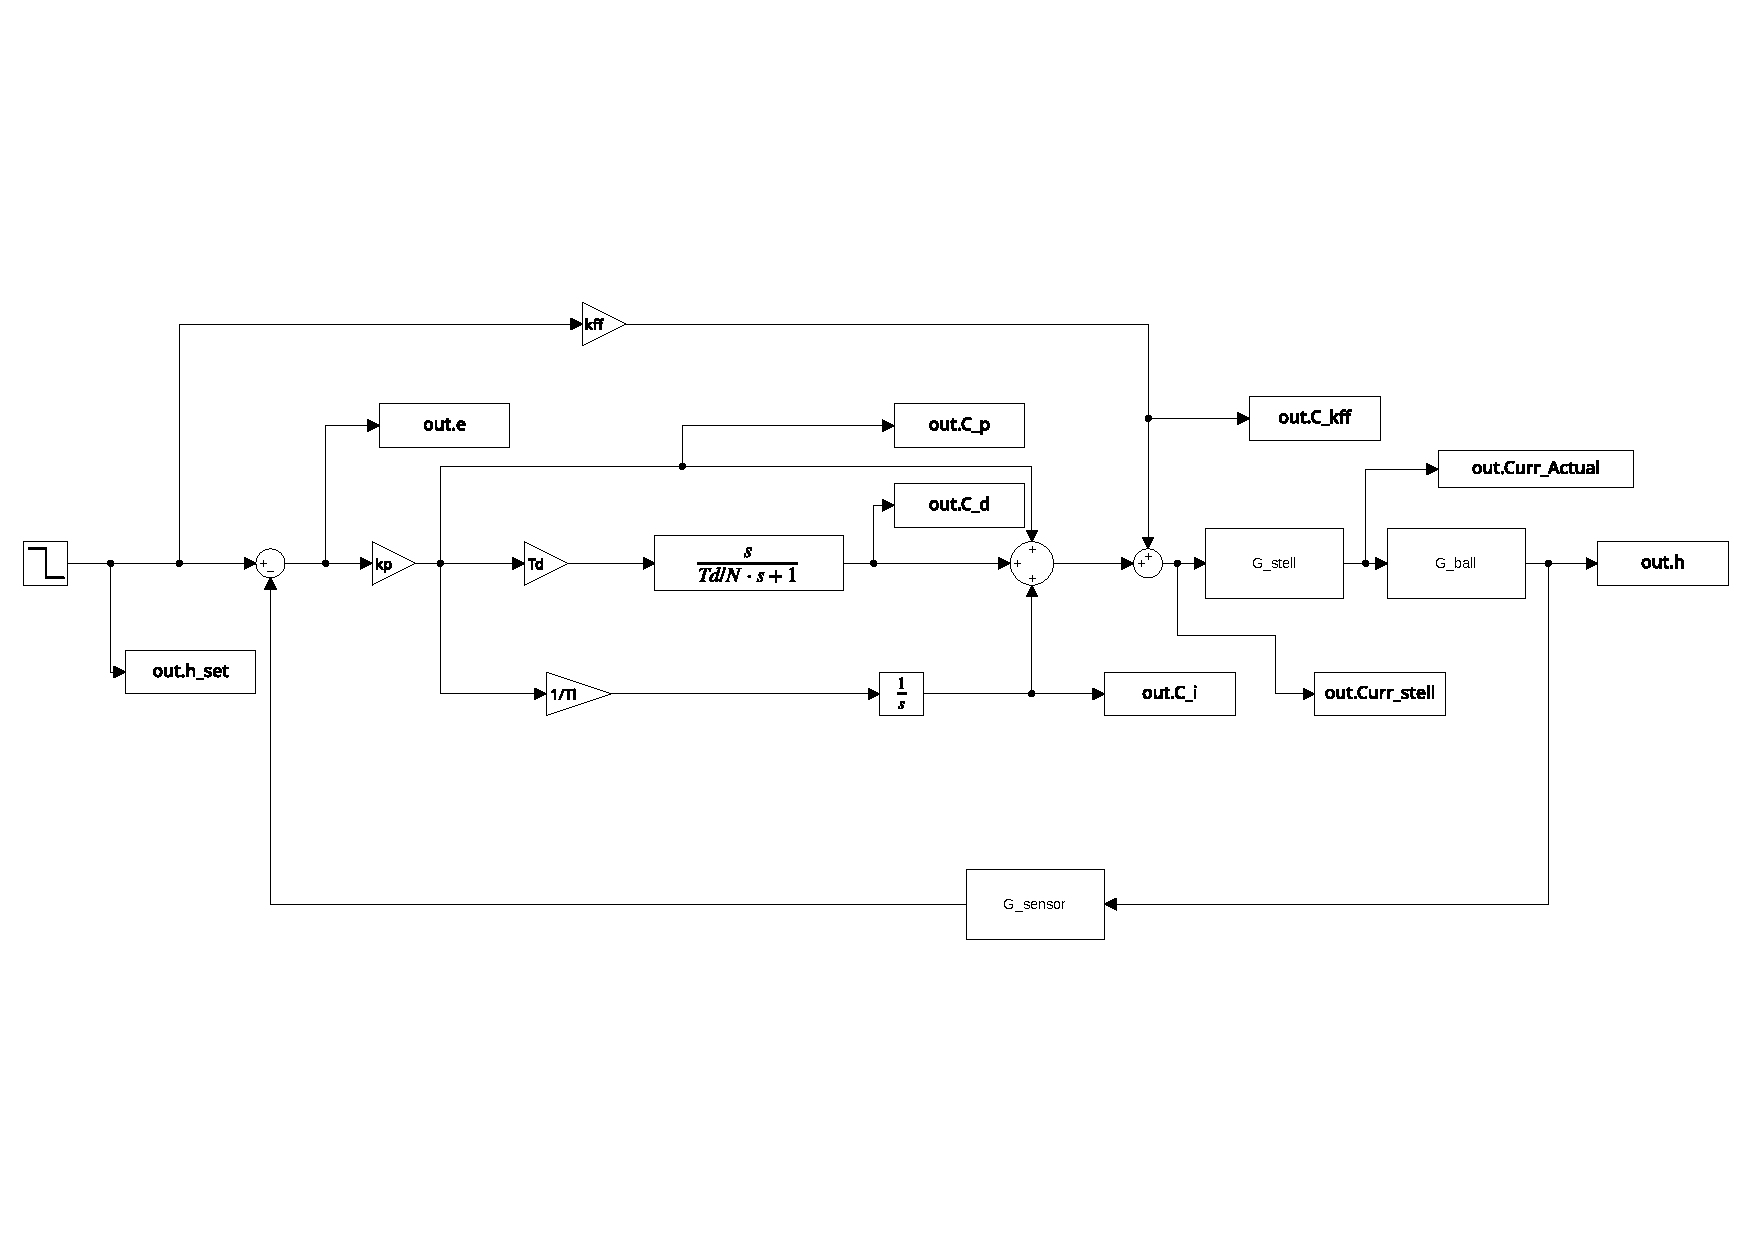
\includegraphics[width=\textwidth]{./figure/magnet_model.pdf}
				\caption{Simulink Modell inlusive Regler-, Stell-, Stecken- und Sensorübertrangungsfunktionen}
				\label{fig:model}
			\end{figure}
\newpage
\section{Aufgabe 17}\label{sec:Aufgabe17}
	\subsection*{Simulation Führungssprung}
	Zunächst wurde der PD-Regler mit einem Führungssprung von $x_0 = 40\si{\milli\meter}$ zu $x_1 = 35\si{\milli\meter}$ simuliert. In \autoref{fig:pd_simu} fällt dabei auf, dass der Regler zwar stabil, aber es scheint ein stationärer Fehler zu entstehen. Dieser Fehler ist ebenfalls weit von dem definierten Arbeitspunkt entfernt, womit der Regler möglicherweise am Versuch nicht funktionieren wird.
			\begin{figure}[H]
				\centering
				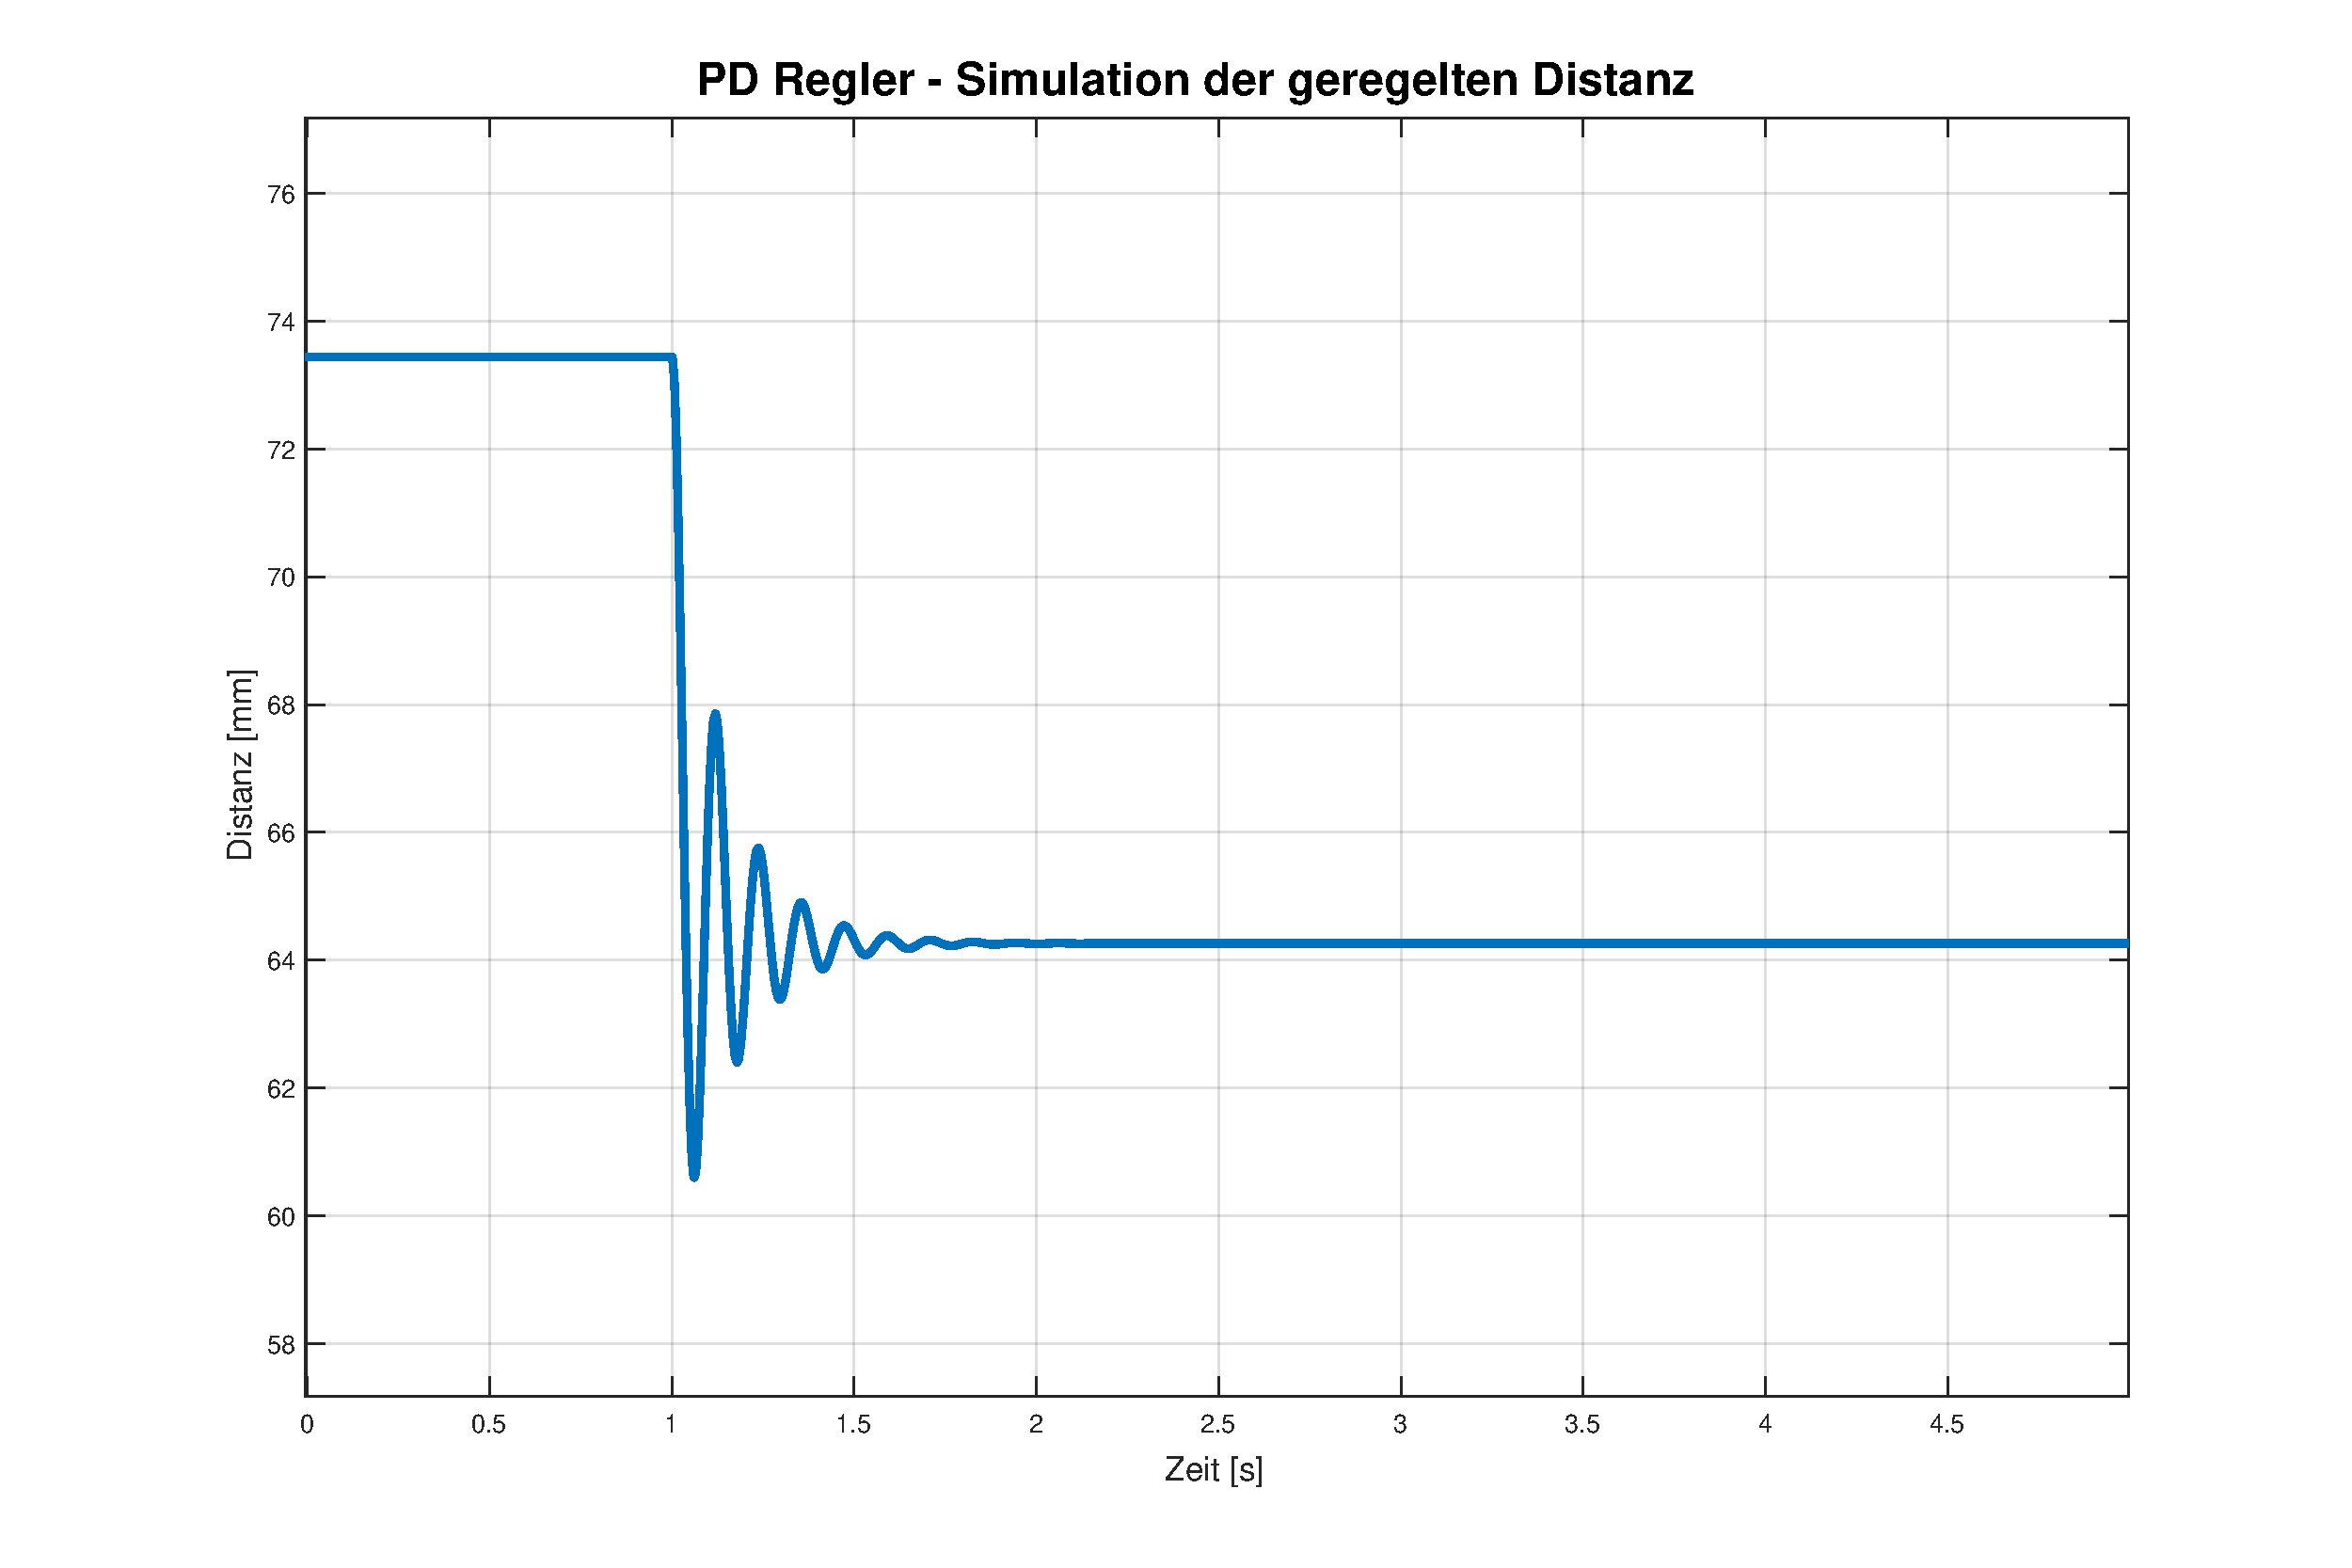
\includegraphics[width=\textwidth]{./figure/PD_simu.pdf}
				\caption{Simulierter Führungssprung mithilfe des PD-Reglers von $x_0 = 40\si{\milli\meter}$ zu $x_1 = 35\si{\milli\meter}$}
				\label{fig:pd_simu}
			\end{figure}


			Wird nun der PD-Regler auf einen PID-Regler erweitert, so stellen sich die gewünschten geregelten Distanzen von   $x_0 = 40\si{\milli\meter}$ zu $x_1 = 35\si{\milli\meter} $ korrekt ein, wie in \autoref{fig:pid_simu}zu sehen ist.
			\begin{figure}[H]
				\centering
				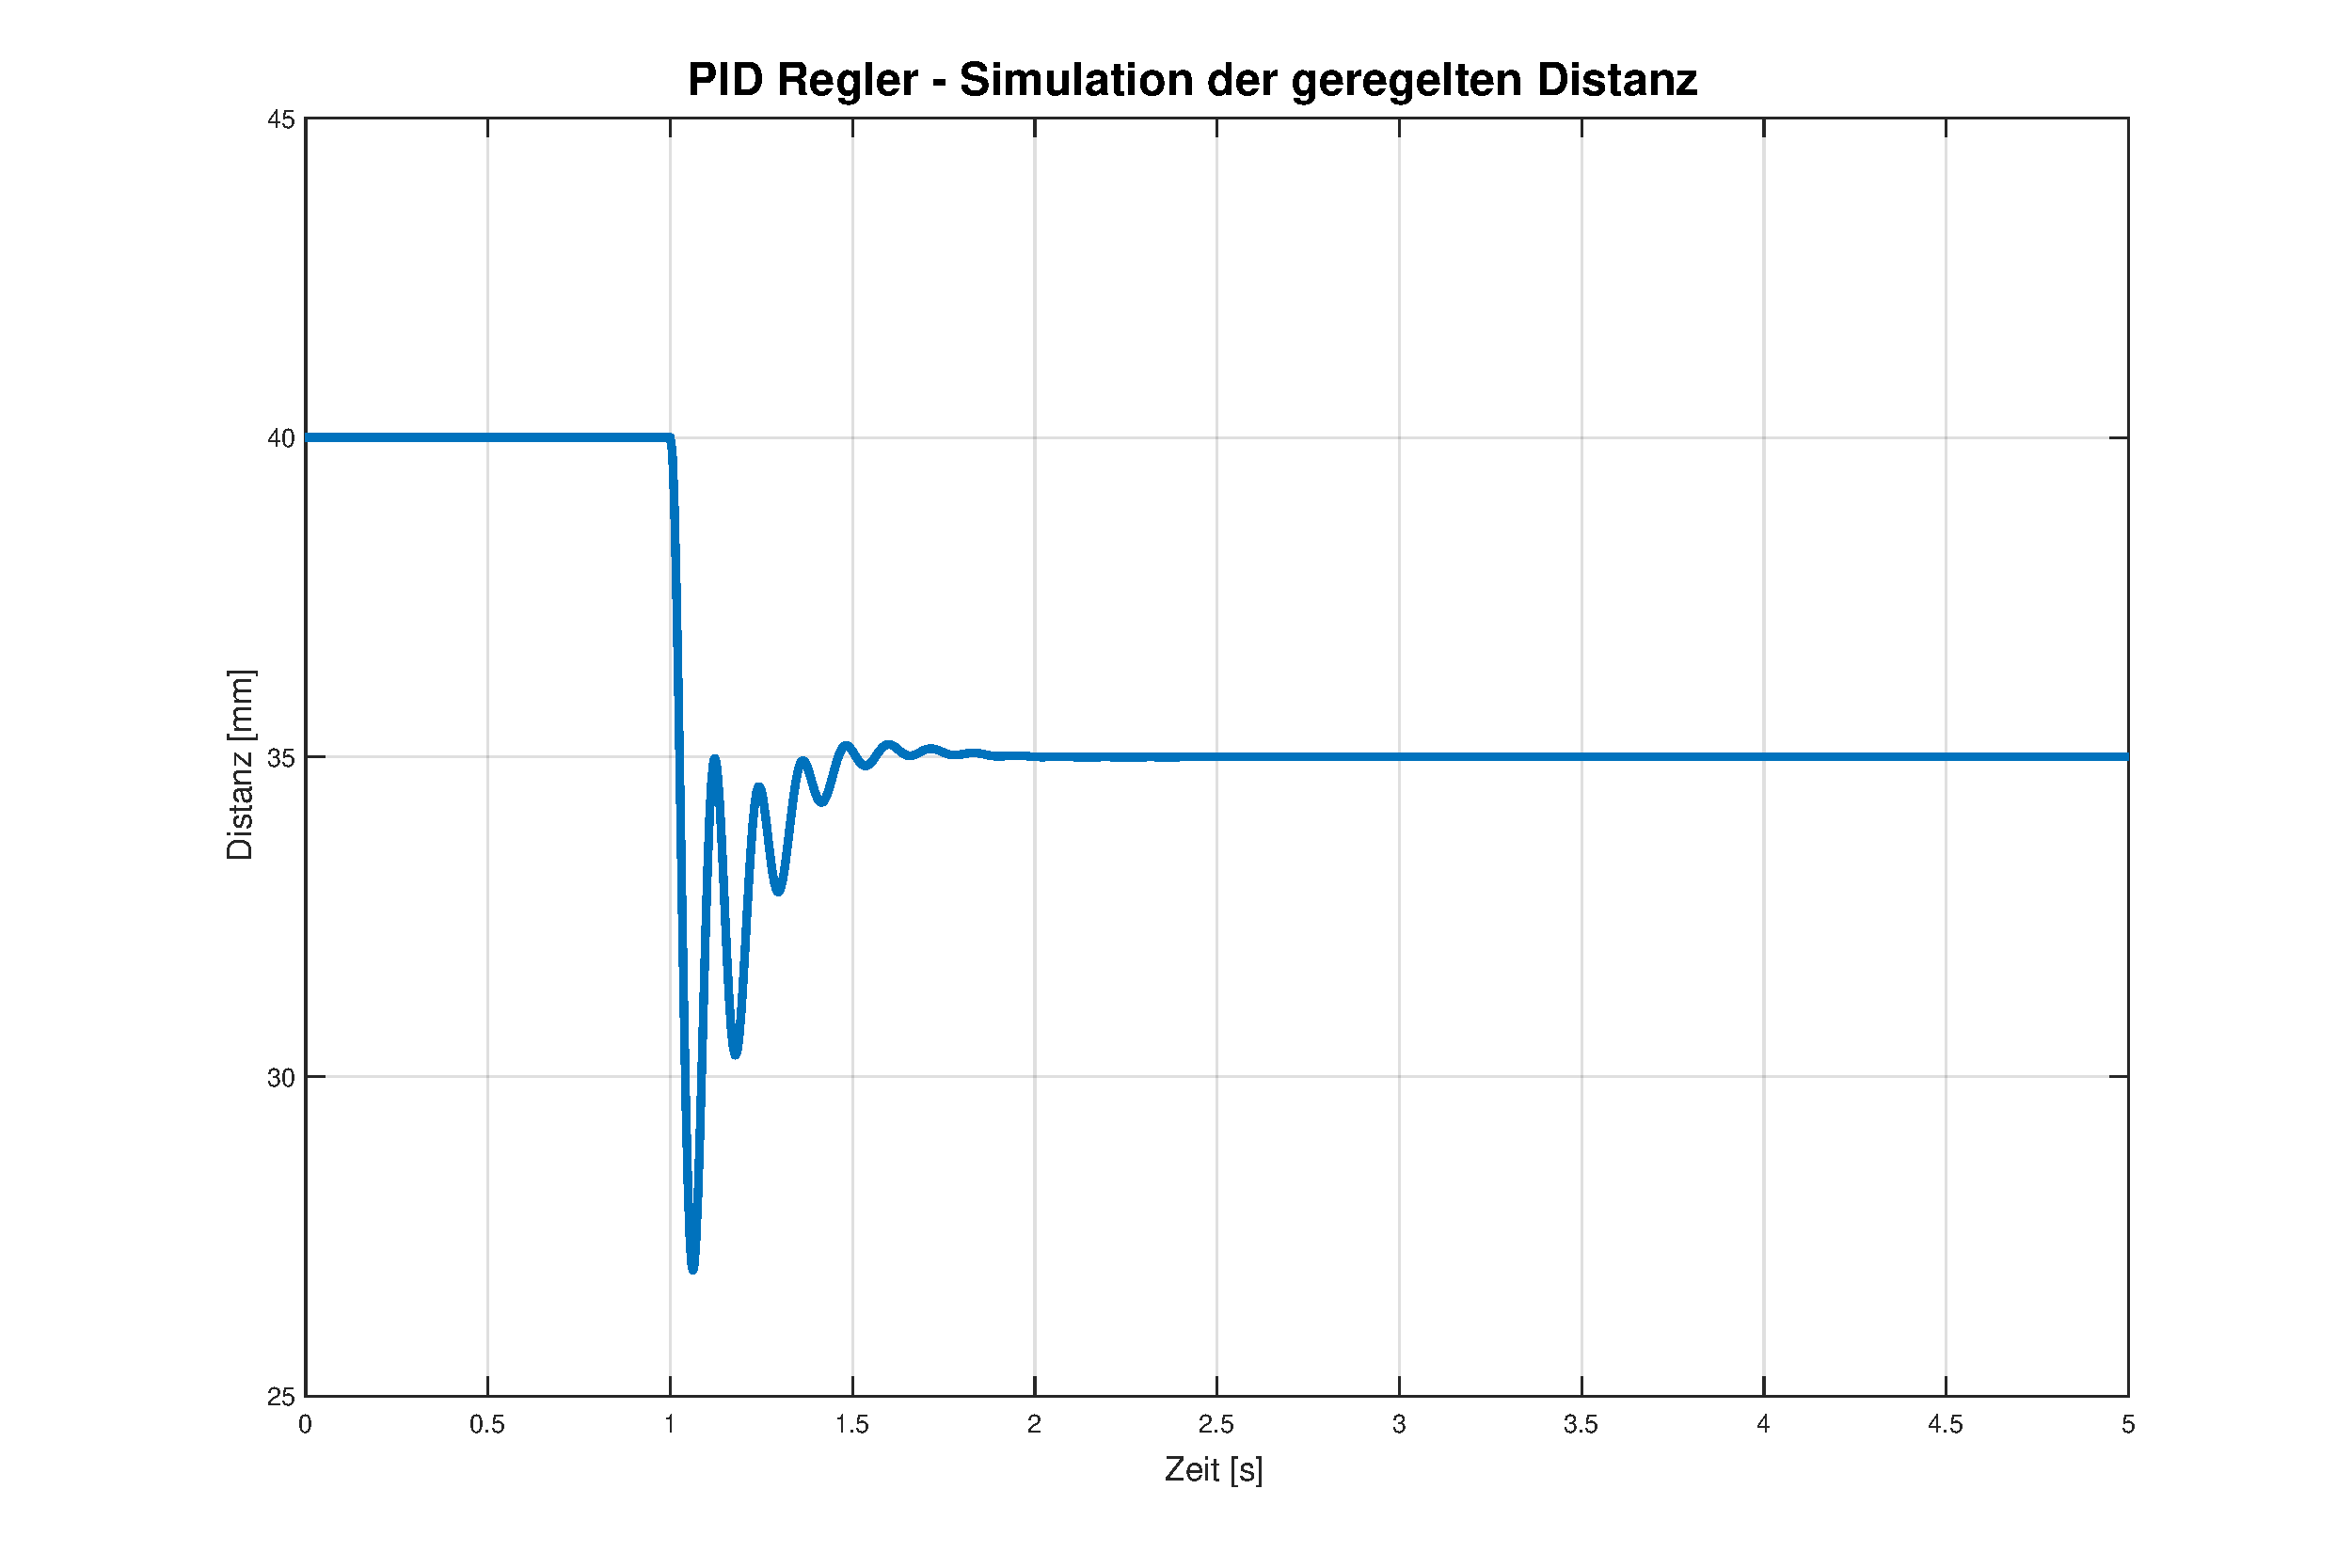
\includegraphics[width=\textwidth]{./figure/PID_simu.pdf}
				\caption{Simulierter Führungssprung mithilfe des PID-Reglers von $x_0 = 40\si{\milli\meter}$ zu $x_1 = 35\si{\milli\meter}$}
				\label{fig:pid_simu}
			\end{figure}
\newpage

\section{Aufgabe 18 und 19}\label{sec:Aufgabe1819}
	\subsection*{Verifikation am Versuch - PD}

	Der PD-Regler hat wie auch in der Simulation ersichtlich einen grossen stationären Fehler. Dies führt dazu, dass er bei $x_{ref}=40\si{\milli\meter}$ eine Distanz von $x_{eff}=60\si{\milli\meter}$ einzunehmen versucht. Dies ist zu weit entfernt, und der Laboraufbau kann nicht genug Strom liefern um den Ball auf Position zu halten. Deshalb wurde der Ball bei $x_0 = 30\si{\milli\meter}$ geregelt, um den simulierten Fehler trotzdem überprüfen zu können.
			
		\begin{figure}[H]
				\centering
				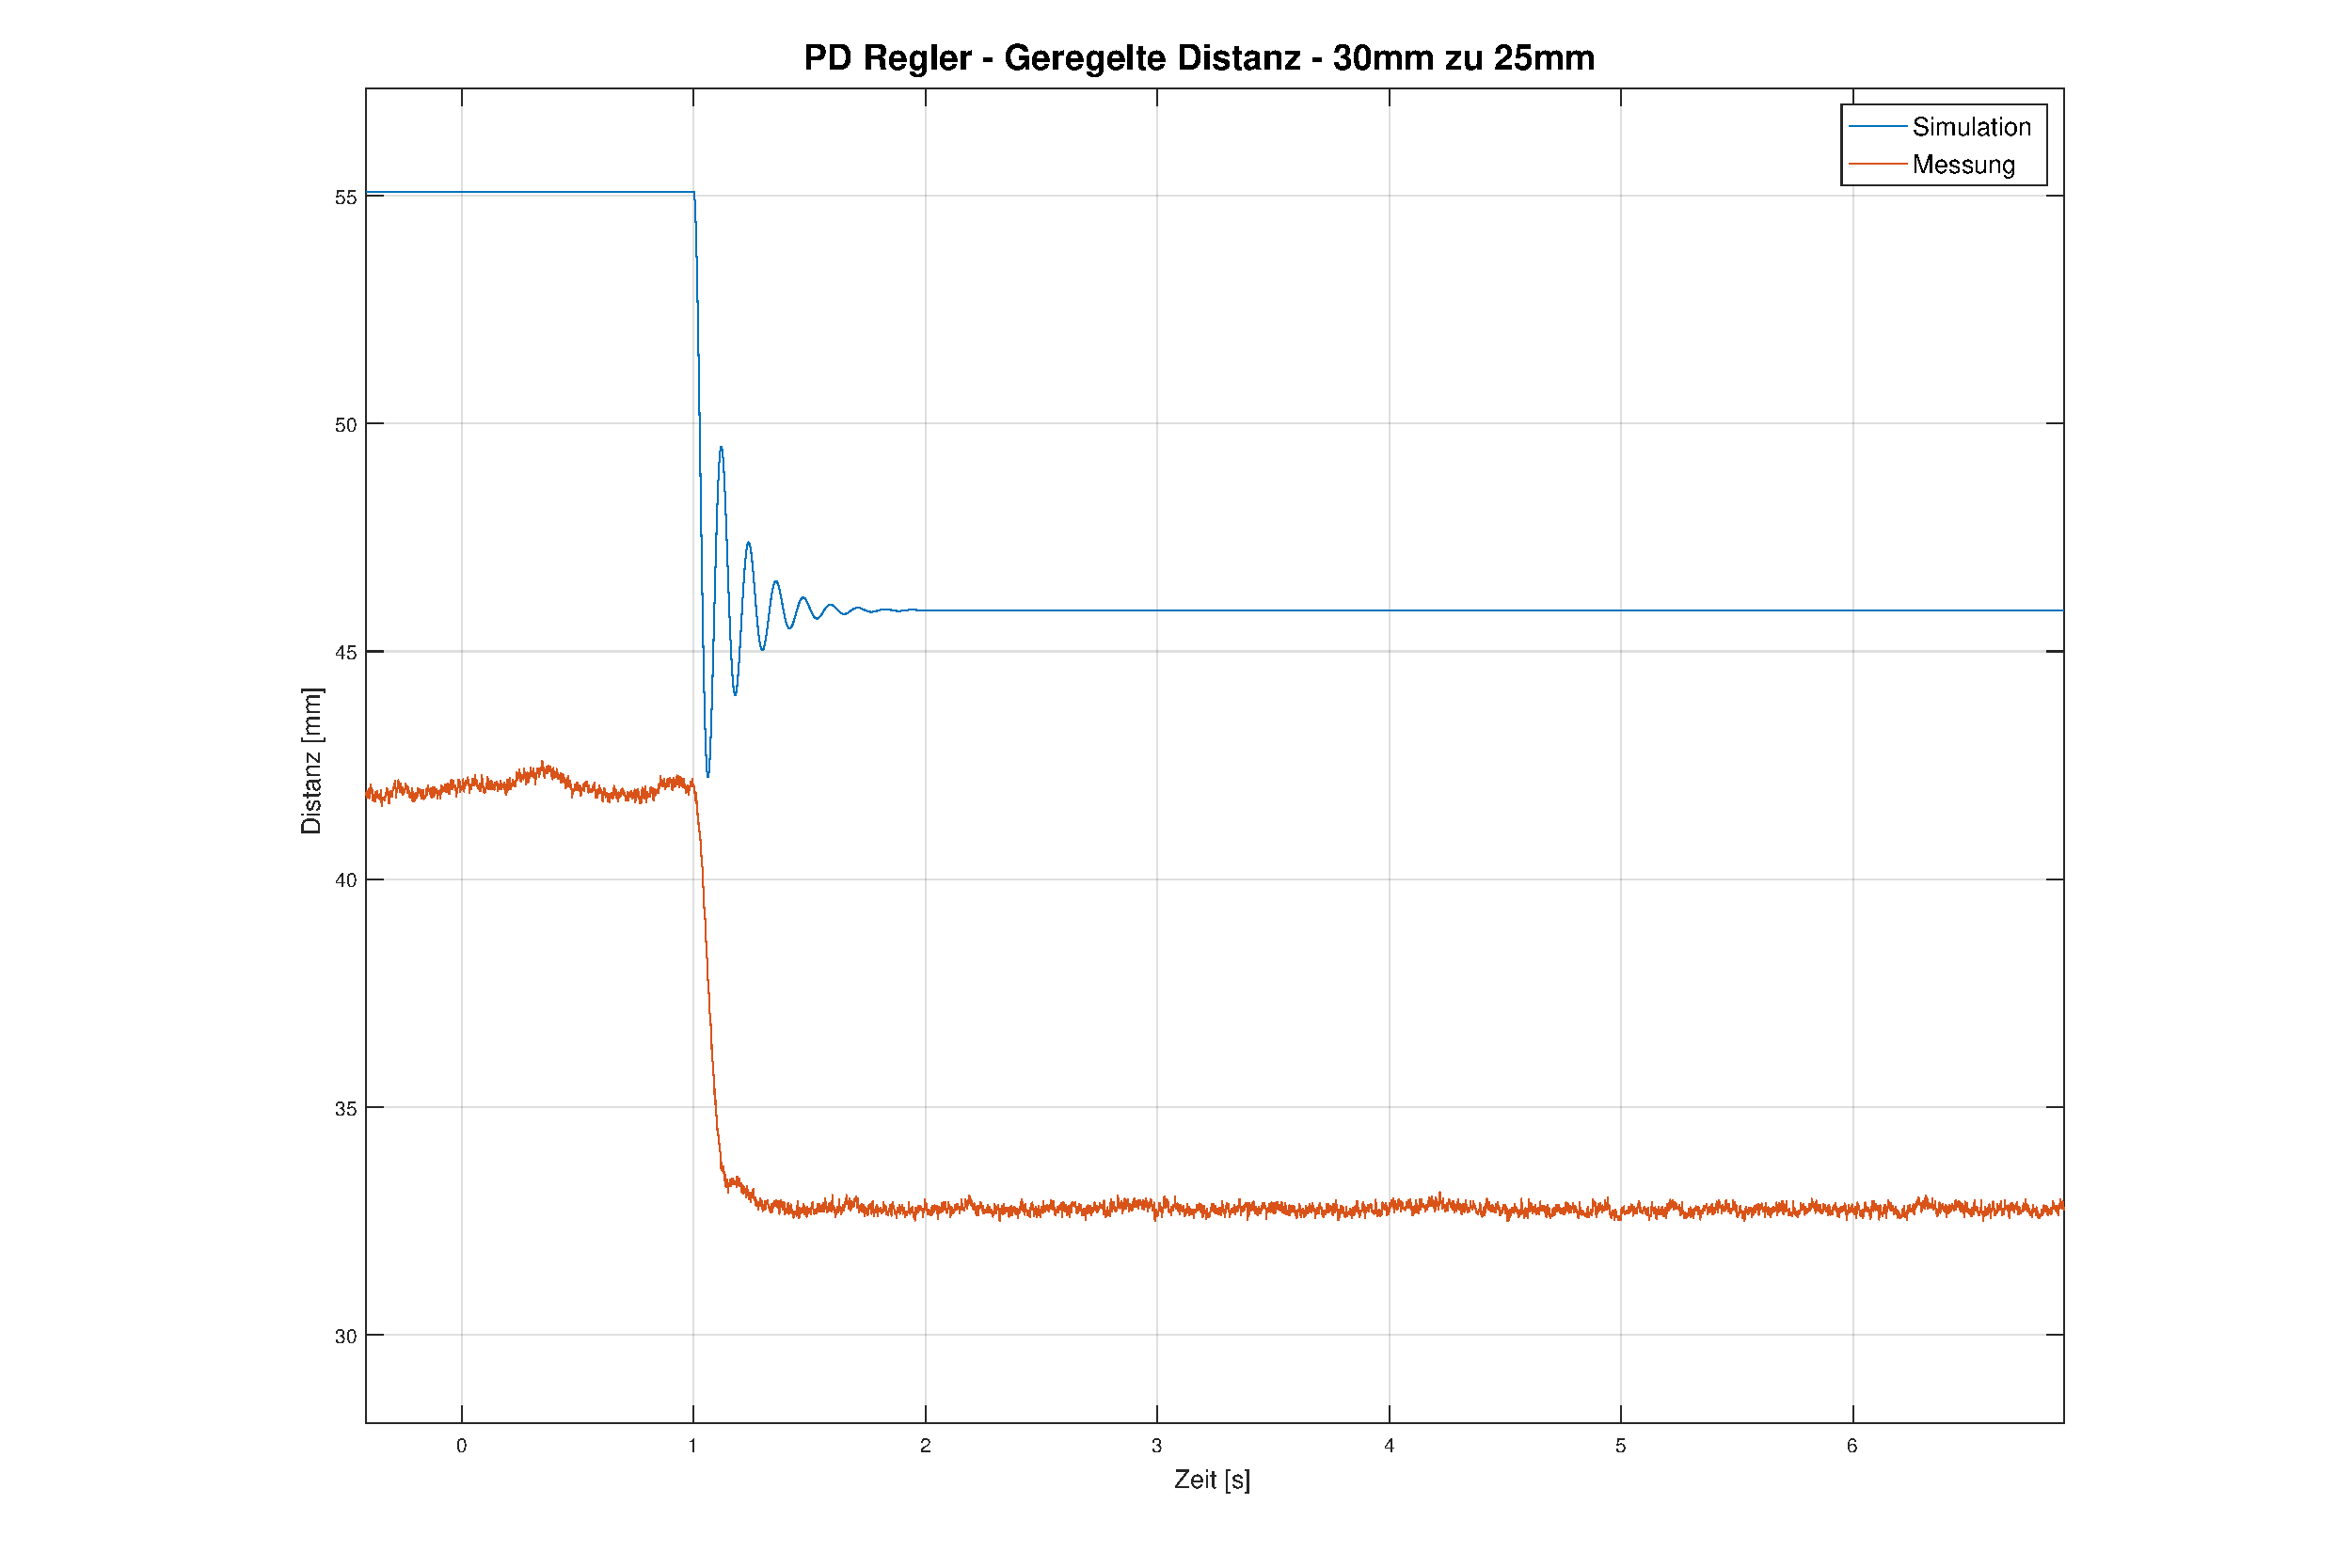
\includegraphics[width=\textwidth]{./figure/PD_mess_distanz.pdf}
				\caption{Simulierter und gemessener Führungssprung mithilfe des PD-Reglers von $x_0 = 30\si{\milli\meter}$ zu $x_1 = 25\si{\milli\meter}$}
				\label{fig:pd_mess}
			\end{figure}
			Hierbei wird in \autoref{fig:pd_mess} beobachtbar, dass laut Simulation der Regelfehler noch viel grösser wird, dies ist auf die weite Distanz zum Arbeitspunkt der Simulation zurückzuführen.

		\begin{figure}[H]
				\centering
				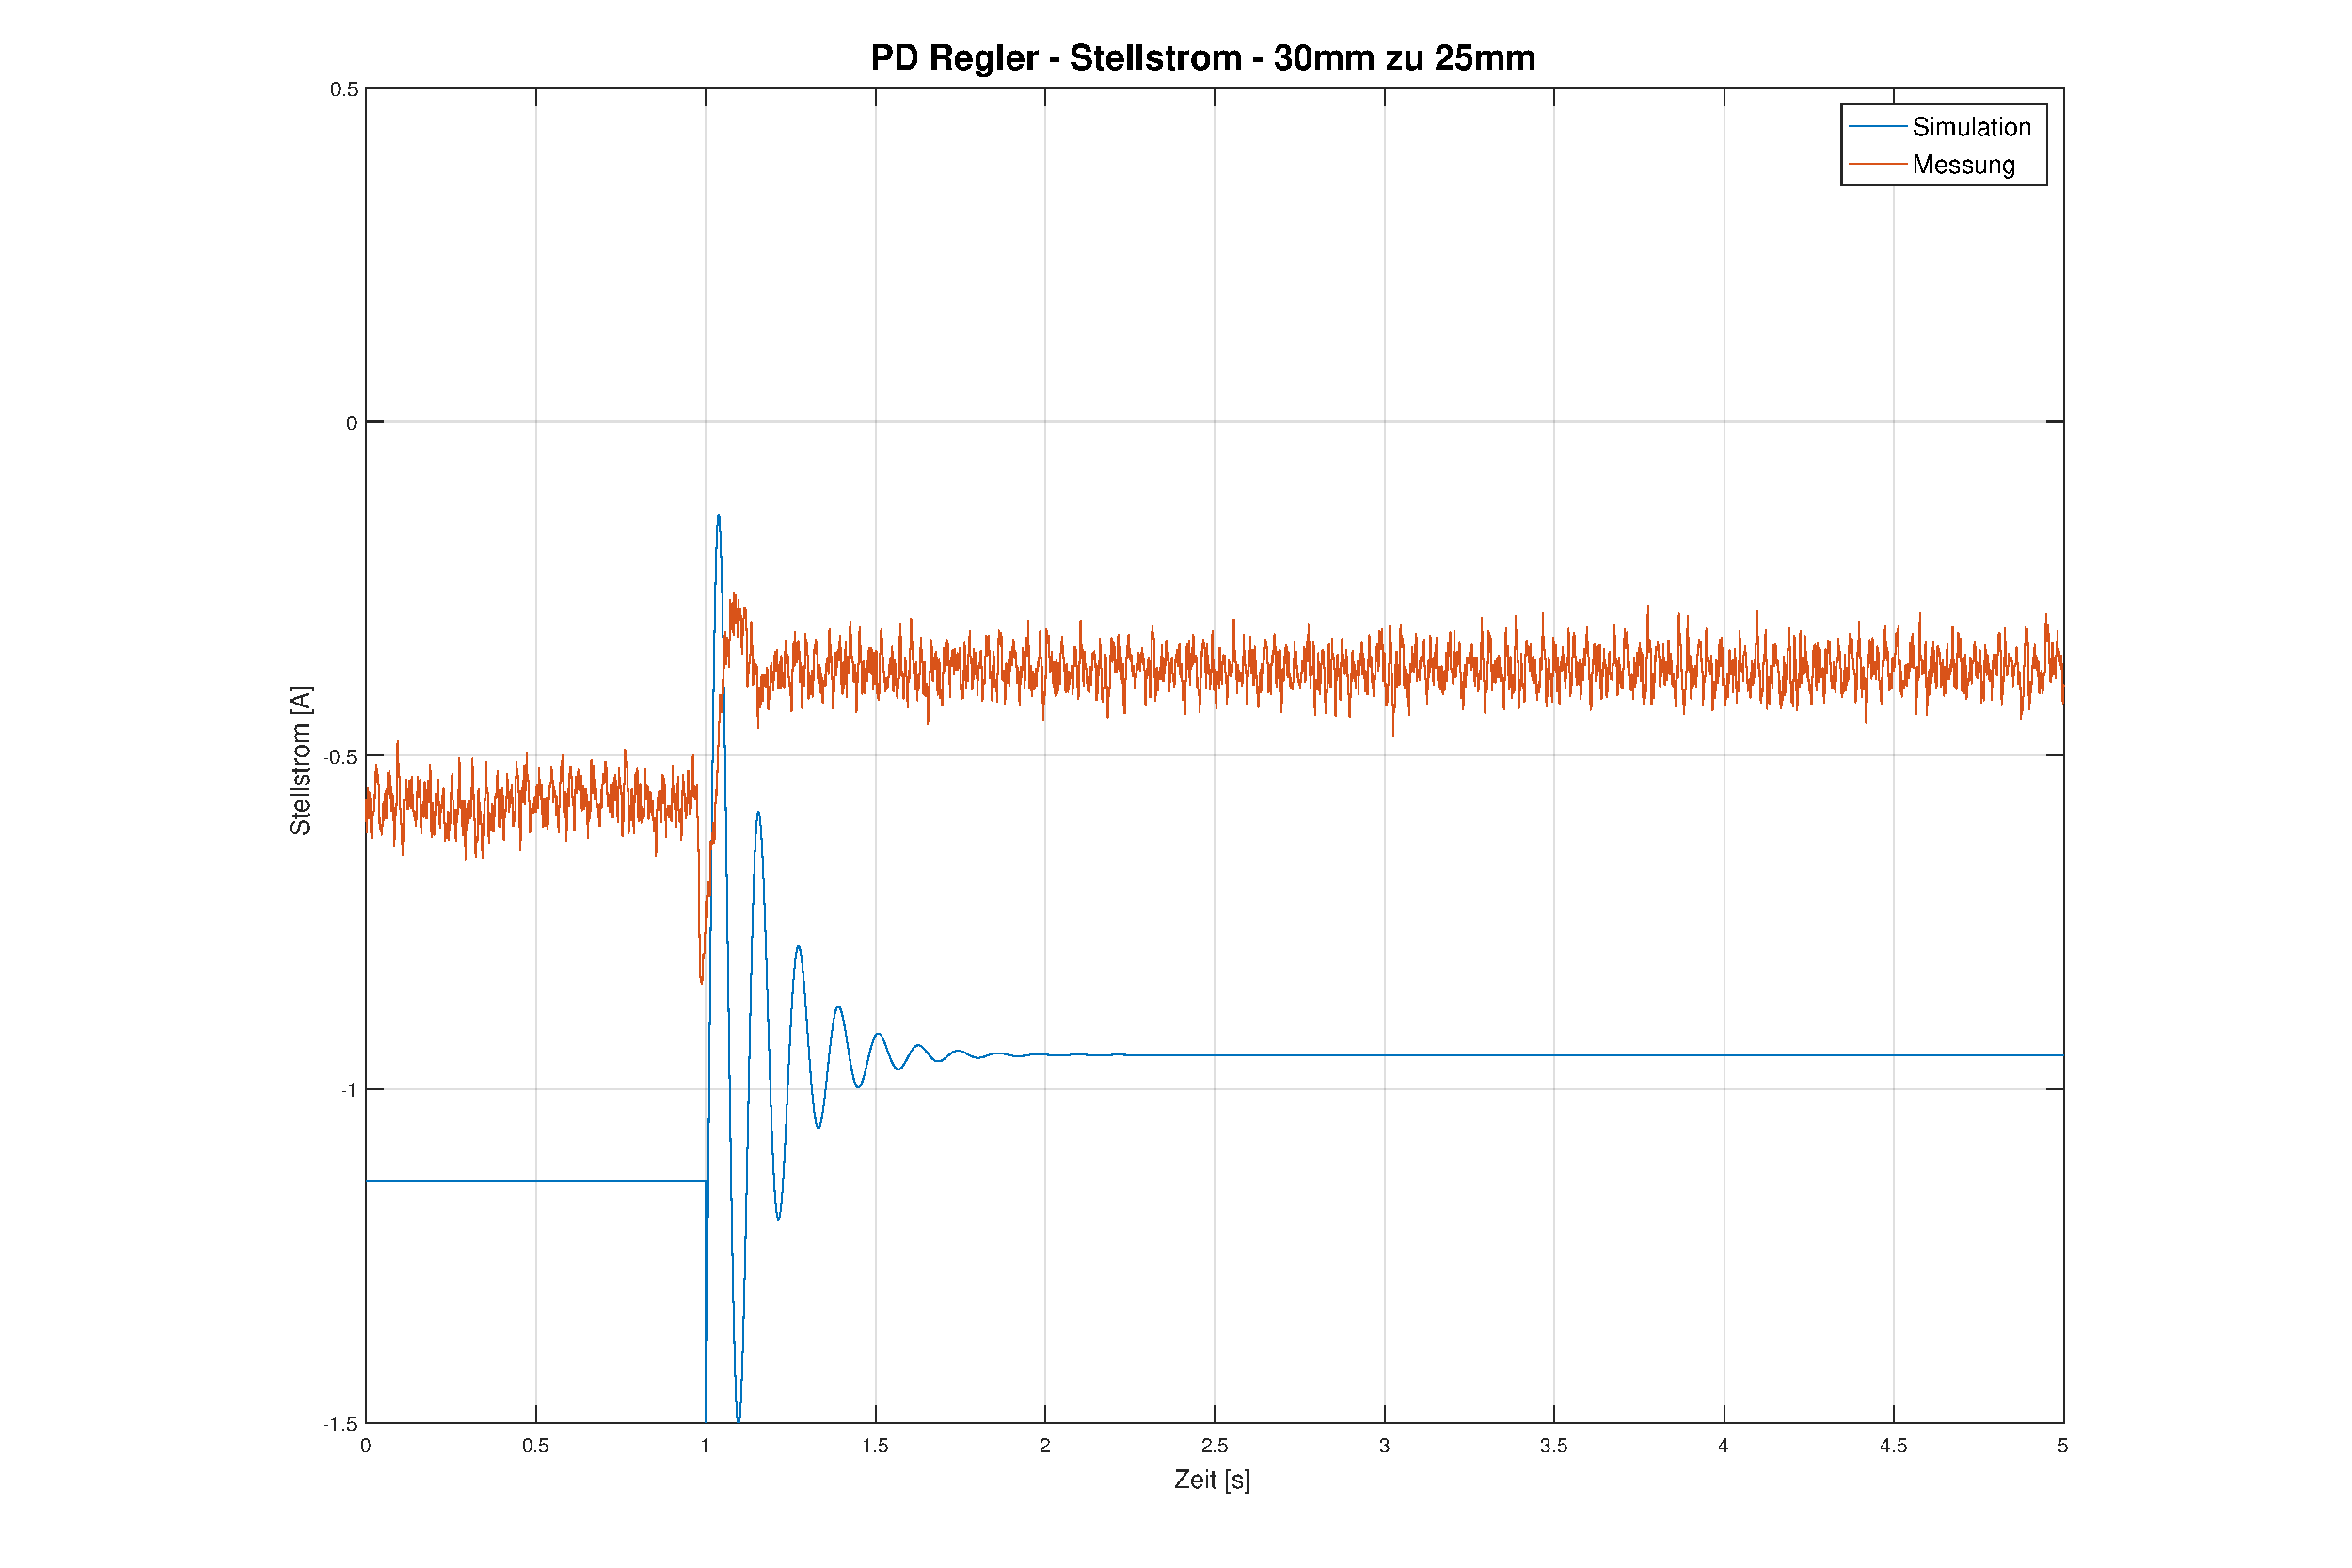
\includegraphics[width=\textwidth]{./figure/PD_mess_stellstrom.pdf}
				\caption{Simulierter und gemessener (SMA(20)) Stellstrom mithilfe des PD-Reglers von $x_0 = 30\si{\milli\meter}$ zu $x_1 = 25\si{\milli\meter}$}
				\label{fig:pd_mess_strom}
			\end{figure}


\newpage 
	\subsection*{Verifikation am Versuch - PID}
	Der PID-Regler hingegen regelt auf die korrekte Soll-Distanz von $x_0 = 40\si{\milli\meter}$ zu $x_1 = 35\si{\milli\meter}$. In \autoref{fig:pid_mess} ist der Vergleich zwischen Simulation und Messung ersichtlich. Erkennbar ist eine hohe Genauigkeit der Simulation bis auf ein nicht vorhandenes Einschwingen der Realität.
			
		\begin{figure}[H]
				\centering
				\includegraphics[width=\textwidth]{./figure/PiD_mess_distanz_40mm.pdf}
				\caption{Simulierter und gemessener Führungssprung mithilfe des PID-Reglers von $x_0 = 40\si{\milli\meter}$ zu $x_1 = 35\si{\milli\meter}$}
				\label{fig:pid_mess}
			\end{figure}
		Auch der Stellstrom in \autoref{fig:pid_mess_strom} ist plausiebler, wenn auch immernoch etwas von der Realität entfernt.
			\begin{figure}[H]
				\centering
				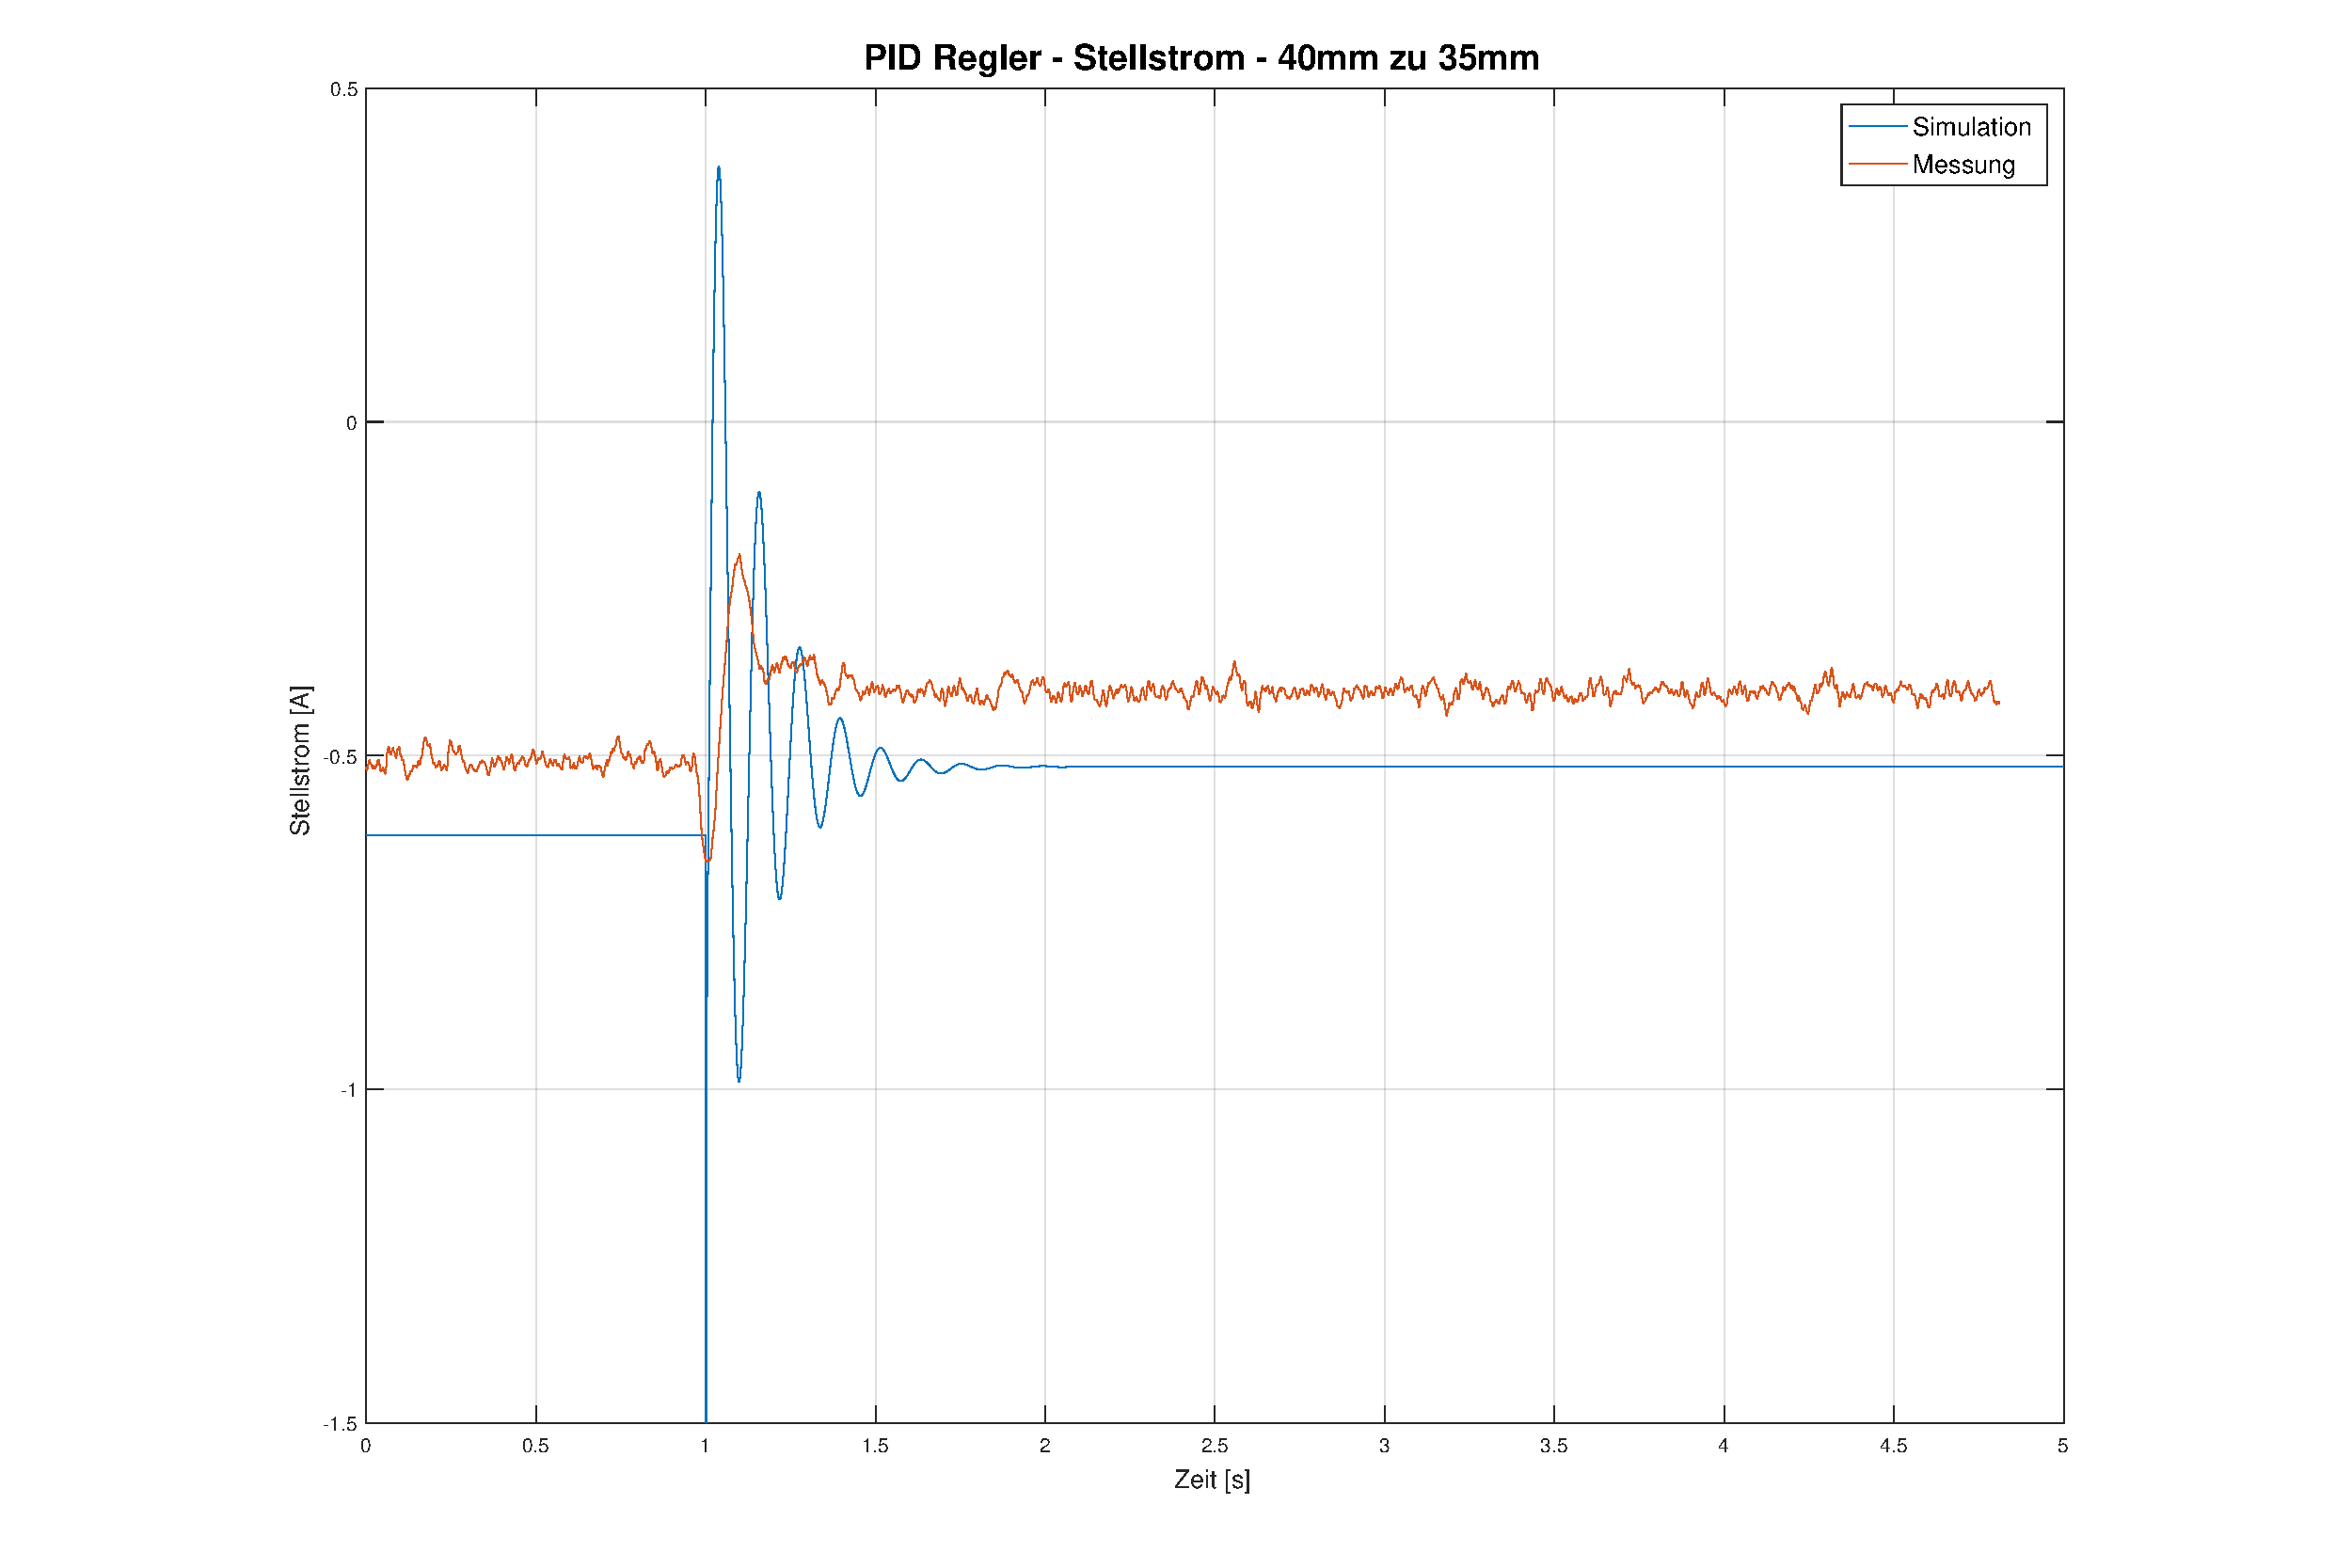
\includegraphics[width=\textwidth]{./figure/PID_mess_stellstrom_40mm.pdf}
				\caption{Simulierter und gemessener (SMA(20)) Stellstrom mithilfe des PID-Reglers von $x_0 = 30\si{\milli\meter}$ zu $x_1 = 25\si{\milli\meter}$}
				\label{fig:pid_mess_strom}
			\end{figure}


\section{Aufgabe 20}\label{sec:Aufgabe20}
	\subsection*{Verbesserung der Regler}
	Mittels Untersuchung der Wurzelortskurve und den Pollagen, wurde ein \textit{guter} PID-Regler entworfen mit den folgenden Paramerten:

		\begin{table}[!h]
			\renewcommand{\arraystretch}{1.2}
			\centering
			\caption{PID Regler Werte}
			\begin{zebratabular}{m{4cm} m{3cm}}
				\rowcolor{gray}
				\textbf{Parameter}	& \textbf{Wert} \\
				$k_p$				& $46$  \\ 
				$T_i$				& $0.3364$  \\
				$T_d$				& $0.0591$ \\
				$N$					& $100$ \\
			\end{zebratabular}
			\renewcommand{\arraystretch}{1.0}
			\label{tab:optimal}
		\end{table}


		\newpage

		Wie in \autoref{tab:optimal_pol} zu erkennen ist, wurden die kritischen Pole (also jene nahe an der Imaginärachse) weiter in den Imaginärteil verschoben, auf kosten der Pole die bereits weit entfernt waren die etwas näher rutschen.
		\begin{table}[!h]
			\renewcommand{\arraystretch}{1.2}
			\centering
			\caption{PID Regler Polunterschied}
			\begin{zebratabular}{m{2cm} m{5cm} m{5cm}}
				\rowcolor{gray}
				\textbf{Pol}	& \textbf{Ursprünglich} & \textbf{Verbessert}\\
				$P_1$				& $(-2.819)10^3$	&			$(-1.6911)10^3$\\
				$P_2$				& $(-0.4080)10^3$	&			$(-0.4138)10^3$\\
				$P_3$				& $(-0.0009 + 0.0377i)10^3$&	$(-0.0070 + 0.0527i)10^3$\\ 
				$P_4$				& $(-0.0009 - 0.0377i)10^3$& 	$(-0.0070 - 0.0527i)10^3$\\ 
				$P_5$				& $(-0.0180)10^3$	&			$(-0.0065 + 0.056i)10^3$\\ 
				$P_6$				& $(-0.0121)10^3$	&			$(-0.0065 - 0.056i)10^3$\\ 
			\end{zebratabular}
			\renewcommand{\arraystretch}{1.0}
			\label{tab:optimal_pol}
		\end{table}


\newpage

\section{Aufgabe 21}\label{sec:Aufgabe21}
	\subsection*{Pole ausserhalb des Arbeitspunkts}
	Wird nun der Arbeitspunkt weit weg vom Linearisierungspunkt gewählt, wandern die Pole wiederum in die rechte Halbebene, was zu einem instabilen Prozess führt.
		\begin{table}[!h]
			\renewcommand{\arraystretch}{1.2}
			\centering
			\caption{Polpositionen bei verschiedenen Arbeitspunkten}
			\begin{zebratabular}{m{4.5cm} m{4.5cm} m{4.5cm}}
				\rowcolor{gray}
				$x_0 = 40\si{\milli\meter}$ &  $x_0 = 30\si{\milli\meter}$ & $x_0 = 50\si{\milli\meter}$\\
				$(-1.6911)10^3$								& $(-1.1678)10^3$	&				$(-1.6918)10^3$\\
				$(-0.4138)10^3$								& $(-0.4647)10^3$	&				$(-0.4046)10^3$\\
				$(-0.0070 + 0.0527i)10^3$					& $(0.0160 + 0.1.235i)10^3$&		$(-0.0320 + 0.0215i)10^3$\\ 
				$(-0.0070 - 0.0527i)10^3$					& $(0.0160 - 0.1235i)10^3$&			$(-0.0320 - 0.0215i)10^3$\\ 
				$(-0.0065 + 0.056i)10^3$					& $(-0.0057 + 0.0057i)10^3$	&		$(0.0269)10^3$\\ 
				$(-0.0065 - 0.056i)10^3$					& $(-0.0057 - 0.0057i)10^3$	&		$(0.0016)10^3$\\ 
			\end{zebratabular}
			\renewcommand{\arraystretch}{1.0}
			\label{tab:optimal_pol}
		\end{table}


